% Definiciones y constantes de estilo
% Clase del documento
\documentclass[a4paper,12pt,twoside,openright,titlepage]{book}

%
% Paquetes necesarios
%

% Símbolo del euro
\usepackage{eurosym}
% Codificación UTF8
\usepackage[utf8]{inputenc}
% Caracteres del español
\usepackage[spanish]{babel}
% Código, algoritmos, etc.
\usepackage{listings}
% Definición de colores
\usepackage{color}
% Extensión del paquete color
\usepackage[table,xcdraw]{xcolor}
% Márgenes
% \usepackage{anysize}
\usepackage[hmargin=3cm,vmargin=3.5cm]{geometry}
% Cabecera y pie de página
\usepackage{fancyhdr}
% Estilo título capítulos
\usepackage{quotchap}
% Algoritmos (expresarlos mejor)
\usepackage{algorithmic}
% Títulos de secciones
\usepackage{titlesec}
% Fórmulas matemáticas
\usepackage[cmex10]{amsmath}
% Enumeraciones
\usepackage{enumerate}
% Páginas en blanco
\usepackage{emptypage}
% Separación entre cajas
\usepackage{float}
% Imágenes
\usepackage[pdftex]{graphicx}
% Mejora de las tablas
\usepackage{array}
% Mejora de los símbolos matemáticos
\usepackage{mdwmath}
% Separar figuras en subfiguras
\usepackage[caption=false,font=footnotesize]{subfig}
% Incluir pdfs externos
\usepackage{pdfpages}
% Mejoras sobre las cajas
\usepackage{fancybox}
% Apéndices
\usepackage{appendix}
% Marcadores (para el pdf)
\usepackage{bookmark}
% Estilo de enumeraciones
\usepackage{enumitem}
% Espacio entre líneas y párrafos
\usepackage{setspace}
% Glosario/Acrónimos
\usepackage[acronym]{glossaries}
% Fuentes
\usepackage[T1]{fontenc}
% Bibliografía
\usepackage[sorting=none,natbib=true,backend=bibtex,bibencoding=ascii]{biblatex}
% Fix biblatex+babel warning
\usepackage{csquotes}

% Enlaces
\hypersetup{hidelinks,pageanchor=true,colorlinks,citecolor=Fuchsia,urlcolor=black,linkcolor=Cerulean}

% Euro (€)
\DeclareUnicodeCharacter{20AC}{\euro}

% Inclusión de gráficos
\graphicspath{{./graphics/}}

% Texto referencias
\addto{\captionsspanish}{\renewcommand{\bibname}{Bibliografía}}

% Extensiones de gráficos
\DeclareGraphicsExtensions{.pdf,.jpeg,.jpg,.png}

% Definiciones de colores (para hidelinks)
\definecolor{LightCyan}{rgb}{0,0,0}
\definecolor{Cerulean}{rgb}{0,0,0}
\definecolor{Fuchsia}{rgb}{0,0,0}

% Keywords (español e inglés)
\def\keywordsEn{\vspace{.5em}
{\textbf{\textit{Key words ---}}\,\relax%
}}
\def\endkeywordsEn{\par}

\def\keywordsEs{\vspace{.5em}
{\textbf{\textit{Palabras clave ---}}\,\relax%
}}
\def\endkeywordsEs{\par}


% Abstract (español e inglés)
\def\abstractEs{\vspace{.5em}
{\textbf{\textit{Resumen ---}}\,\relax%
}}
\def\endabstractEs{\par}

\def\abstractEn{\vspace{.5em}
{\textbf{\textit{Abstract ---}}\,\relax%
}}
\def\endabstractEn{\par}

% Estilo páginas de capítulos
\fancypagestyle{plain}{
\fancyhf{}
%\fancyfoot[CO]{\footnotesize\emph{\nombretrabajo}}
\fancyfoot[CO]{\thepage}
%\fancyfoot[RO]{\thepage}
\renewcommand{\footrulewidth}{.6pt}
\renewcommand{\headrulewidth}{0.0pt}
}

% Estilo resto de páginas
\pagestyle{fancy}

% Estilo páginas impares
%\fancyfoot[CO]{\footnotesize\emph{\nombretrabajo}}
\fancyfoot[CO]{\thepage}
\rhead[]{\leftmark}

% Estilo páginas pares
%\fancyfoot[CE]{\emph{\pieparcen}}
\fancyfoot[CE]{\thepage}
%\fancyfoot[RE]{\pieparizq}
\lhead[\leftmark]{}

% Guía del pie de página
\renewcommand{\footrulewidth}{.6pt}

% Nombre de los bloques de código
\renewcommand{\lstlistingname}{Código}

% Estilo de los lstlistings
\lstset{
    frame=tb,
    breaklines=true,
    postbreak=\raisebox{0ex}[0ex][0ex]{\ensuremath{\color{gray}\hookrightarrow\space}}
}

% Definiciones de funciones para los títulos
\newlength\salto
\setlength{\salto}{3.5ex plus 1ex minus .2ex}
\newlength\resalto
\setlength{\resalto}{2.3ex plus.2ex}

% Estilo de los acrónimos
\renewcommand{\acronymname}{Glosario}
\renewcommand{\glossaryname}{Glosario}
\pretolerance=2000
\tolerance=3000

% Texto índice de tablas
\addto\captionsspanish{
\def\tablename{Tabla}
\def\listtablename{\'Indice de tablas}
}

% Traducir appendix/appendices
\renewcommand\appendixtocname{Apéndices}
\renewcommand\appendixpagename{Apéndices}

% Comando code (lstlisting sin cambio de página)
\lstnewenvironment{code}[1][]%
  { \noindent\minipage{0.935\linewidth}\medskip
    \vspace{5mm}
    \lstset{basicstyle=\ttfamily\footnotesize,#1}}
  {\endminipage}


% Definiciones de comandos
\newcommand{\nombreautor}{TODO: Nombre del Autor}
\newcommand{\nombredirector}{TODO: Nombre del director}
\newcommand{\nombretrabajo}{TODO: Título de la Tesis Fin de Máster}
\newcommand{\fecha}{\today}
\newcommand{\lugar}{Madrid}
\newcommand{\master}{Máster Universitario en Ingeligencia Artificial}
% Descomentar si tu trabajo tiene un co-director
%\newcommand{\nombrecodirector}{TODO: Nombre del co-director}
% Descomentar si tu trabajo está asociado a un grupo de investigación
% \newcommand{\grupoInvestigacion}{TODO: Grupo de investigación}
\newcommand{\departamento}{TODO: Departamento}
\newcommand{\facultad}{Escuela Técnica Superior de Ingenieros Informáticos}
\newcommand{\universidad}{Universidad Politécnica de Madrid}
\newcommand{\pieparizq}{TODO: Pie de página par}
\newcommand{\pieparcen}{Master Thesis}
\newcommand{\logoizq}{logo_politecnica}
\newcommand{\logoder}{logo_informatica}
\newcommand{\correo}{TODO: Correo de contacto}


% Glosario y acrónimos
\makeglossaries
\input{src/glosario}

% Rerefencias
\bibliography{src/bibliografia}

% Inicio del documento
\begin{document}

% Elección del idioma (español)
\selectlanguage{spanish}

%
% Portada
%
\pagenumbering{gobble}
%
% Portada
%

\begin{titlepage}
  
\includepdf{portada_jaime}
\end{titlepage}
% \hypersetup{pageanchor=true}

\pagenumbering{roman}

% Estilo de párrafo de los capítulos
\setlength{\parskip}{0.75em}
\renewcommand{\baselinestretch}{1.25}
% Interlineado simple
\spacing{1}

%
% Agradecimientos
%

\include{src/dedicatoria}
\include{src/agradecimientos}

%
% Resumen
%
\pagenumbering{roman}
\setcounter{page}{0}
% Resumen en español
\chapter*{Resumen}

\begin{abstractEs}
	Hoy en día, la Web tiende a ser un espacio interactivo donde la comunicación entre un cliente y un servidor web es bidireccional y la información se mueve en tiempo real. Este cambio puede reflejarse en los teléfonos móviles, con la explosión de las apps de mensajería instantánea que ofrecen una nueva forma de comunicación a través del envío de mensajes de texto gratuitos.

	Muchas empresas han apostado por remodelar sus servicios para aprovecharse de los beneficios de las tecnologías en tiempo real, debido a que ahora existen herramientas que nos facilitan enormemente este proceso y ya supone un gran esfuerzo.

	Pero los centros 112 de Europa todavía no se han aprovechado de estas nuevas tendencias. Hasta este momento, solo ofrecen la posibilidad de comunicarte con los servicios de emergencias a través de llamadas de voz, y a través de sus apps gratuitas, el envío de la ubicación actual del ciudadano y, si es necesario, de fotografías para agilizar una primera intervención.

	Ante esta situación, los proveedores de PSAPs deberían contemplar la integración de las tecnologías en tiempo real, para recibir no solo voz, sino también texto en tiempo real, ficheros multimedia, videollamadas u otra información relevante. Y de este modo, proveer un acceso universal como a ciudadanos con algún tipo de discapacidad que les impide realizar una llamada al 112 en condiciones.

	A lo largo de este documento, con el objetivo de mejorar la respuesta de los servicios de emergencias, se describe el estudio de nuevas alternativas tecnologías en tiempo real y el desarrollo de una solución software con baja complejidad de integración y cuyo rendimiento cumpla con los requisitos impuestos por los centros 112.

\end{abstractEs}

% Palabras clave en español
\begin{keywordsEs}
	mensajería instantánea, app, Centro 112, PSAP
\end{keywordsEs}

% Resumen en inglés
\chapter*{Abstract}

\begin{abstractEn}
TODO: Resumen en inglés, 250-500 palabras.

\end{abstractEn}

% Palabras clave en inglés
\begin{keywordsEn}
TODO: Palabras clave en inglés, separadas por coma.
\end{keywordsEn}




%
% Glosario
%
%\printglossary[title=Glosario,toctitle=Glosario]
%\printglossary[title=Acrónimos,toctitle=Acrónimos,type=\acronymtype]

% Estilo de párrafo de los índices
\setlength{\parskip}{1pt}
\renewcommand{\baselinestretch}{1}

%
% Tabla de contenidos
%
\tableofcontents
\listoffigures
\listoftables
\cleardoublepage

% Estilo de párrafo de los capítulos
\setlength{\parskip}{0.75em}
\renewcommand{\baselinestretch}{1.25}
% Interlineado simple
\spacing{1}
% Numeración contenido
\pagenumbering{arabic}
\setcounter{page}{1}

%
% Introducción
%
\chapter{INTRODUCCIÓN}

Internet ha sufrido una evolución radical desde sus inicios. A día de hoy, la Web tiende a ser un espacio interactivo en el cual la comunicación entre un cliente y un servidor web es bidireccional y la información se mueve en tiempo real.

Este gran cambio puede reflejarse en los teléfonos móviles, con la explosión de las apps de mensajería instantánea. Estas apps permiten el envío de mensajes de texto gratuitos a través de Internet. También ofrecen opciones de voz y video, y la posibilidad de compartir archivos.

Pero las apps que permiten comunicarnos con los servicios de emergencias no han evolucionado con la misma rapidez que la tecnología en tiempo real. Estas apps hasta ahora, solo permiten enviar de forma automática la ubicación actual a las centros de emergencias y, si es necesario, enviar fotografías para agilizar una primera intervención.

\clearpage

\section{Motivaciones del proyecto}

El mundo del desarrollo web avanza rápido, cada día surgen nuevas herramientas y nuevas tendencias que debemos implementar si queremos seguir siendo competitivos dentro del mercado. El presente de las aplicaciones web, se podría afirmar que es la respuesta inmediata, lo que en tecnología se conoce como tiempo real.

Estos últimos años, las empresas han apostado por remodelar sus productos para aprovecharse de los beneficios de las aplicaciones web en tiempo real. Esto se debe a que integrar la funcionalidad de tiempo real supone un gran esfuerzo, pero ahora existen herramientas que nos facilitan enormemente este proceso.

Node.js es una de estas herramientas que en los últimos tiempos ha alcanzado una popularidad innegable, hasta llegar a ser un componente indispensable en el desarrollo de aplicaciones web.

Por otra parte, la mensajería instantánea, que ha evolucionado desde los años 90, hoy en día se ha sofisticado y adoptado como parte del uso cotidiano. Las compañías, las organizaciones políticas y otras entidades están utilizando cada vez más la mensajería instantánea como medio para comunicarse con los clientes e incluso, entre compañeros de trabajo.

Pero los centros 112 de Europa todavía no se han aprovechado de estas nuevas tendencias que han revolucionado el Internet. Las apps de emergencias, solo ofrecen la posibilidad de comunicarte con los servicios de emergencias a través de llamadas de voz.

Siendo conscientes de esto, algunos centros de emergencias, buscan incluir aquellas novedades tecnológicas que sean fáciles de incorporar a corto plazo. Con el objetivo de ofrecer una mejor respuesta de los servicios de emergencias y una nueva alternativa de comunicación en tiempo real.

\section{Objetivos del proyecto}

A día de hoy, los ciudadanos usan todos los días comunicaciones basadas en IP, como la mensajería instantánea, y sería interesante la posibilidad de comunicarse con los servicios de emergencias utilizando estos medios. Pero la organización del 112 y los servicios de emergencias solo son accesibles mediante llamadas telefónicas de voz.

Motivo más que suficiente para que los PSAPs cambien su tecnología para ser parte del futuro; es decir, mejorar sus sistemas de emergencias con la integración de las tecnologías en tiempo real, para recibir no solo voz, sino también información de ubicación, texto en tiempo real, ficheros multimedia o videollamadas.

Por esta razón, el trabajo plantea el estudio de las nuevas soluciones y tecnologías disponibles que puedan mejorar los sistemas de emergencias. Y posteriormente, llevar a cabo el desarrollo de un solución software en tiempo real con un baja complejidad de integración. No obstante, al tratarse de un nuevo servicio en los sistemas de emergencias es de vital importancia realizar un análisis del rendimiento y el coste del mismo.

%
% Estado del arte
%
\chapter{ESTADO DEL ARTE\label{sec:estado_del_arte}}

\clearpage

Las tendencias tecnológicas siguen evolucionando y cada día van apareciendo nuevos conceptos que debemos aprender.

\section{Servicios de emergencia}

Desde 1998, los países de la Unión Europea tienen la obligación de garantizar que los usuarios de teléfonos fijos y móviles puedan llamar sin coste alguno al número de emergencia 112 para comunicar una incidencia de cualquier tipo.

Si la llamada se hace a través de un teléfono fijo, el centro de atención de emergencias conocerá desde dónde se ha realizado la llamada. Pero si se llama desde un teléfono móvil, sólo se podrá saber la zona desde donde más o menos se hace la llamada, en ningún caso el punto exacto en el que se encuentra quien requiere la ayuda.

\subsection{Número de emergencia europeo}

El gran aumento de los viajeros dentro de la Unión Europea hizo que el Consejo de la Unión Europea decidiera introducir un número de emergencia común en todos los estados para evitar la necesidad de recordar diferentes números nacionales dependiendo de la ubicación.

\begin{figure}[htp!]
  \centering
  
\includegraphics[scale=0.05,clip=true]{112_logo}
  \caption{112, número de emergencia europeo}
  \label{fig:112_logo}
\end{figure}

Este número de emergencia europeo fue el 112 y, desde entonces, se encuentra disponible de forma gratuita, 24 horas al día, los 365 días al año, en cualquier lugar de la Unión Europea. Un ciudadano puede marcar el 112 para comunicarse con los servicios de emergencia, incluida también la policía, los servicios de asistencia médica y el cuerpo de bomberos.

La llamada de emergencia a un centro 112 puede realizarse aunque no se disponga de cobertura del operador de red que estemos usando, pero sí de algún otro, pues se utiliza la red GSM (Global System for Mobile communications) que haya disponible. El teléfono móvil realiza la llamada de voz igualmente si se desconoce el PIN e incluso si el teléfono no tiene introducida la tarjeta SIM en el terminal o la pantalla está bloqueada.

\subsection{EENA}

La Asociación del Número de Emergencia Europeo o EENA (acrónimo en inglés de European Emergency Number Association) cree que tener un número de emergencia común en todas partes de Europa está beneficiando directamente a los ciudadanos y visitantes pero desafortunadamente, este número que puede salvar vidas es en gran parte desconocido.

\begin{figure}[htp!]
  \centering
  
\includegraphics[scale=0.4,clip=true]{eena_logo}
  \caption{Logo de EENA}
  \label{fig:eena_logo}
\end{figure}

EENA es una organización sin ánimo de lucro con base en Bruselas y establecida en 1999 con el objetivo de promover servicios de emergencia de calidad a través del número de emergencia 112 en toda Europa. Esta organización proporciona una plataforma de intercambio de información y experiencias entre los servicios de emergencia, autoridades públicas, investigadores y la industria de la tecnología con el objetivo de mejorar la respuesta a las situaciones de emergencia de acuerdo a los requisitos de los usuarios.

EENA, basándose en diferentes fuentes, ha diseñado los modelos 112. Los modelos 112 no cubren todo el modelo de manejo de llamadas, sino que intentan resaltar sus características principales. Los modelos 112 no presentan todos los modelos sobre la organización de los PSAPs (Public Safety Answering Point) en Europa, pero presentan los conceptos principales con descripciones simplificadas.

\subsubsection{Modelo donde las EROs atienden las llamadas}

En este modelo las llamadas a números nacionales y al 112 son redirigidas a las  Organizaciones de Respuesta de Emergencia (ERO, acrónimo en inglés de Emergency Response Organisation). Si se requiere la intervención de una ERO diferente, la llamada y/o los datos sobre la situación de emergencia se envían a la ERO más adecuada. En una variante, dos EROS son colocadas y contactadas a través del mismo número.

\begin{figure}[htp!]
  \centering
  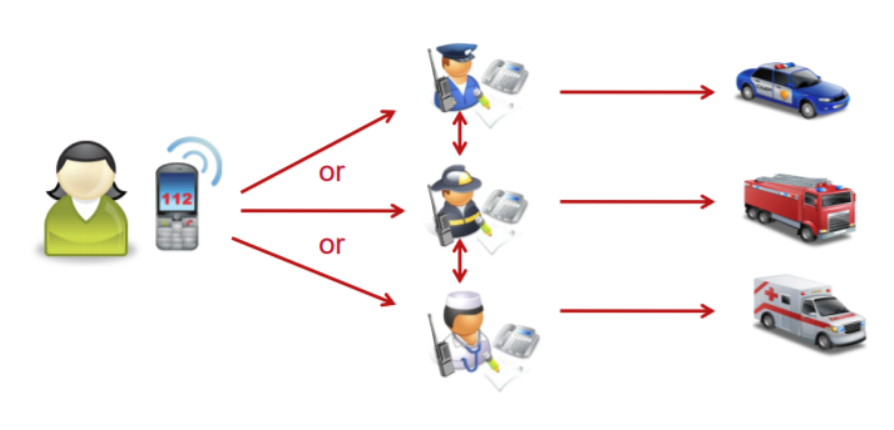
\includegraphics[width=0.75\textwidth,clip=true]{modelo112_1}
  \caption{Modelo 112 de Austria, Francia, Alemania e Italia}
  \label{fig:modelo112_1}
\end{figure}

\subsubsection{Modelo de filtrado de llamadas y envío de recursos}

En este modelo las llamadas a números nacionales y al 112 son redirigidas a las  Organizaciones de Respuesta de Emergencia (ERO, acrónimo en inglés de Emergency Response Organisation). Si se requiere la intervención de una ERO diferente, la llamada y/o los datos sobre la situación de emergencia se envían a la ERO más adecuada. En una variante, dos EROS son colocadas y contactadas a través del mismo número.

\begin{figure}[htp!]
  \centering
  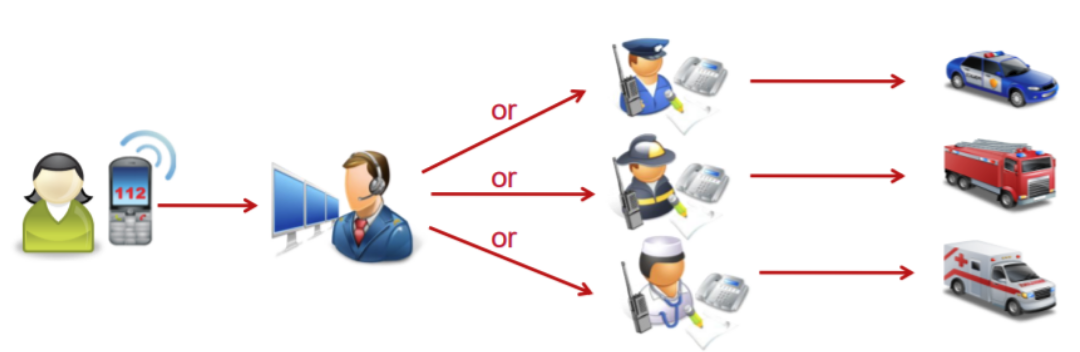
\includegraphics[width=0.75\textwidth,clip=true]{modelo112_2}
  \caption{Modelo 112 de Reino Unido e Irlanda}
  \label{fig:modelo112_2}
\end{figure}

\subsubsection{Modelo de recogida de datos y envío de recursos}

La diferencia respecto al modelo 2 es el papel que juegan las organizaciones independientes. Los operadores clasifican la llamada y hacen un envio paralelo de las llamadas a las EROs. En algunos casos, los especialistas de las EROs están disponibles para dar soporte a los operadores. Las EROs se encargan del envío de los recursos de intervención.

\begin{figure}[htp!]
  \centering
  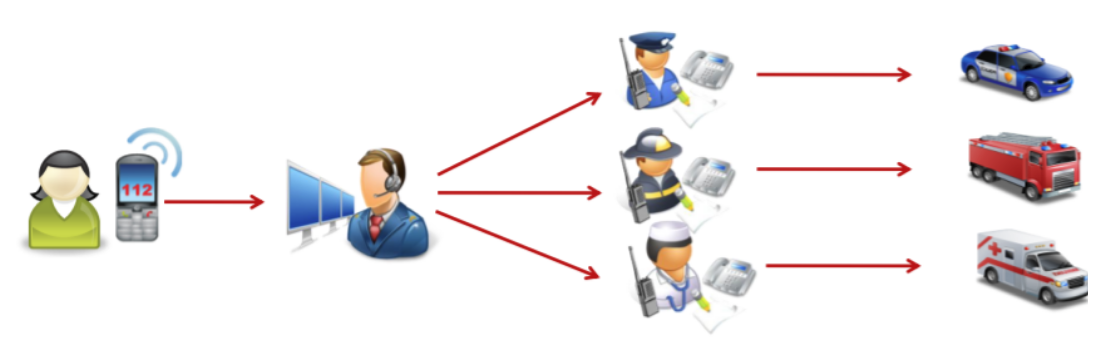
\includegraphics[width=0.75\textwidth,clip=true]{modelo112_3}
  \caption{Modelo 112 de Rumanía}
  \label{fig:modelo112_3}
\end{figure}

\subsubsection{Modelo de recogida de datos y envío de recursos en la misma sala de control}

Este modelo también se realiza en dos niveles. Los operadores y las EROs se encuentran en el mismo lugar. Los operadores están a cargo de clasificar la llamada y, en el caso que sea necesario, hacer un envio paralelo de las llamadas a las EROs más apropiadas. En algunos casos, los especialistas de las EROs están disponibles para dar soporte a los operadores. Las EROs se encargan del envío los recursos de intervención.

\begin{figure}[htp!]
  \centering
  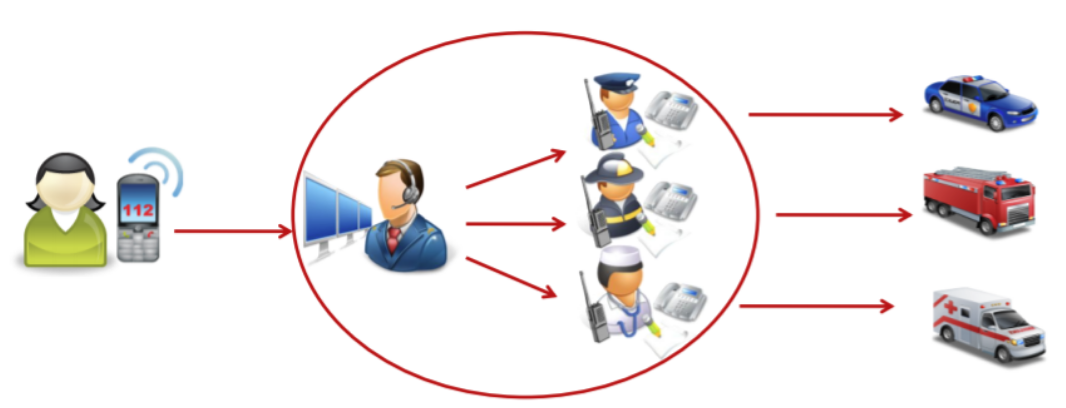
\includegraphics[width=0.75\textwidth,clip=true]{modelo112_4}
  \caption{Modelo 112 de algunas Comunidades Autónomas de España, Bélgica y Túrquia}
  \label{fig:modelo112_4}
\end{figure}

\subsubsection{Modelo donde las EROs y el PSAP son independientes}

En este modelo, los operadores se hacen cargo tanto de la atención de las llamadas como del envío de los recursos de intervención. En algunos casos, los especialistas de las EROs están disponibles para dar soporte a los operadores. El mismo PSAP se encarga de la clasificación de las llamadas, la recogida de datos y el envío de los recursos de intervención a la incidencia.

\begin{figure}[htp!]
  \centering
  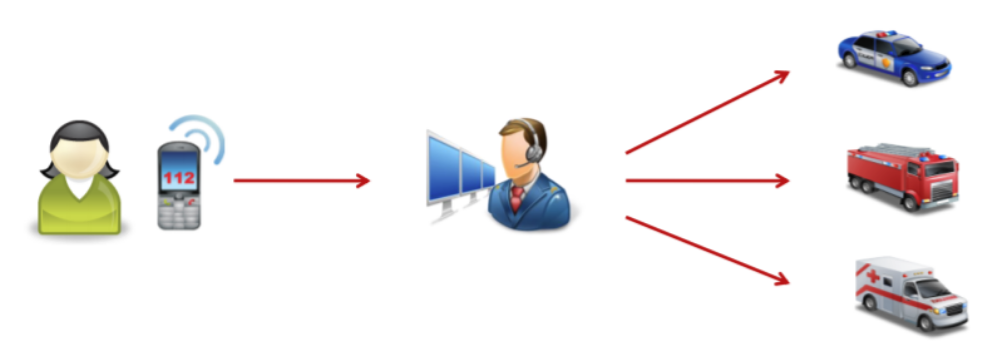
\includegraphics[width=0.75\textwidth,clip=true]{modelo112_5}
  \caption{Modelo 112 de Finlandia}
  \label{fig:modelo112_5}
\end{figure}

\subsubsection{Modelo donde las PSAPs están interconectados}

Los PSAP de diferentes regiones se pueden interconectar. Si no hay disponible un operador, la llamada puede ser redirigida a otro PSAP.

\begin{figure}[htp!]
  \centering
  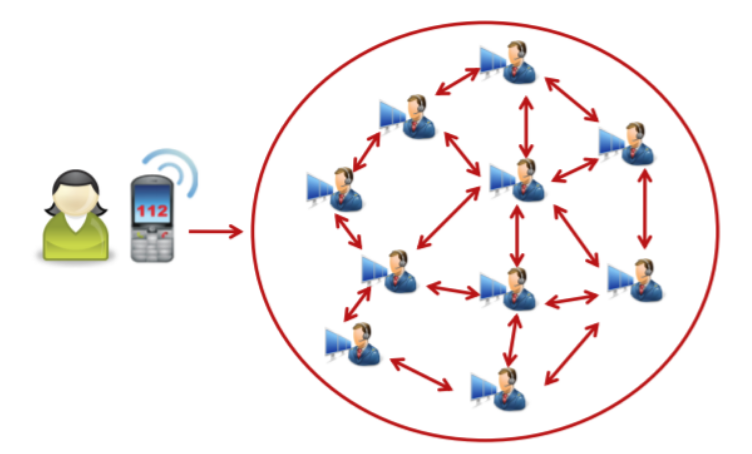
\includegraphics[width=0.75\textwidth]{modelo112_6}
  \caption{Modelo 112 de Bulgaria, República Checa y Suecia}
  \label{fig:modelo112_6}
\end{figure}

\subsection{Centro 112 de Madrid}

El teléfono 112 se activó en la Comunidad de Madrid el 1 de enero de 1998 para atender, tratar y evaluar todas las llamadas de emergencia de los madrileños. Ese año recibió alrededor de un millón de llamadas. A día de hoy, la cifra supera los 86,6 millones, lo que lo consagra como una gran central de gestión de emergencias que ofrece confianza y seguridad a los ciudadanos.

\begin{figure}[htp!]
  \centering
  
\includegraphics[scale=0.3,clip=true]{madrid112_logo}
  \caption{Logo de Madrid 112}
  \label{fig:madrid112_logo}
\end{figure}

El Centro 112 de Madrid está diseñado bajo un criterio multiservicio que permite integrar operativamente a todos los organismos de emergencia, mediante los acuerdos precisos para definir los procedimientos que determinan cuándo hay que activar cada servicio. Todo ello, con independencia de que se encuentren integrados físicamente en el Centro 112, como sucede con los principales, o que sus sedes estén ubicadas fuera del Centro.

El Centro 112 de la Comunidad de Madrid, ha incorporado en su Sistema Integrado de Gestión de Emergencias (SIGE112) una novedosa aplicación móvil permitiendo la localización del llamante mediante las coordenadas desde donde se está realizando la llamada.

El trabajo de los profesionales, junto con el desarrollo tecnológico, sirve para optimizar la asistencia y para que la gestión del 112 de la Comunidad de Madrid haya obtenido la norma ISO 22320, siendo el único de España en tener este certificado de calidad.

\subsubsection{Modelo Madrid 112}

Los procedimientos determinan también los intercambios de información necesarios para conocer en todo momento el desarrollo de la gestión de la incidencia. Este tipo de modelo, determina que el trabajo se desarrolle a dos niveles:

\begin{enumerate}
  \item \textbf{Recepción, atención y gestión de la llamada}. Este proceso corresponde a Madrid 112 y tiene por finalidad, partiendo de la información de cada llamada, activar los servicios precisos que tienen que resolver la emergencia.
  \item \textbf{Movilización y gestión de recursos}. Corresponde a los organismos de intervención directa en la emergencia la activación de los recursos adecuados para la resolución de la emergencia. La actividad operativa que corresponde a Madrid 112 se desarrolla fundamentalmente en la sala de operaciones.
\end{enumerate}

El modelo de Madrid 112 está diseñado con criterios de escalabilidad que nos permiten ir incorporando los avances de las nuevas tecnologías.

\subsubsection{Atributos de la plataforma tecnológica}

La plataforma tecnológica goza de una serie de atributos, al objeto de brindar un soporte eficaz a la gestión de las emergencias, tales como:

\begin{itemize}
  \item \textbf{Capacidad}, para atender la potencial demanda de emergencias de los más de 6 millones de ciudadanos existentes en el ámbito territorial de la Comunidad de Madrid. Número al que se deben añadir las personas en tránsito y turistas. El Centro 112 goza de un excedente de capacidad, espacial, operativa y tecnológica para poder hacer frente a casos extremos de catástrofe o gran emergencia, a sabiendas de que lo que funciona bien en el régimen ordinario, lo hará también en el extraordinario.
  \item \textbf{Seguridad}, entendida como el aseguramiento de la prestación continuada del Servicio 24 h/día, 365 días/año. Este aseguramiento se sustenta en que el suministro de energía está garantizado mediante doble acometida exterior y la existencia de grupos electrógenos con capacidad de soportar y redundar las necesidades energéticas del Centro. El aseguramiento de las comunicaciones y la información se soporta en la redundancia de elementos críticos de los sistemas, y en la existencia de un centro de respaldo del principal.
  \item \textbf{Flexibilidad e integrabilidad}, características que toman cuerpo en la existencia de un sistema de integración radiotelefónica, capaz de integrar redes de radio de distinta tecnología que conviven en la Comunidad de Madrid y facilitando la interoperabilidad de todos los efectivos de emergencia que actúan en nuestra Comunidad.
\end{itemize}

\section{Servicios de emergencia de nueva generación}

En 20 países es posible acceder los servicios de emergencia a través de SMS al 112, incluido en España. También se puede en Bélgica, Croacia, Estonia, Finlandia, Francia, Irlanda, Letonia, Lituania, Luxemburgo, Rumanía, Eslovenia, Suecia y Reino Unido. También se puede, pero sólo a través de un número más largo, en Austria, Chipre, Dinamarca, Italia, Malta y Portugal.

A día de hoy, los ciudadanos tienen la necesidad de comunicarse con los servicios de emergencias a través de los medios que utilizan diariamente, y la organización del 112 y los servicios de emergencias están muy dispersos en toda la Unión Europa y aun más en el mundo entero.

Los distintos PSAPs deben afrontarse a ciertos cambios, que tienen un impacto directo en sus organizaciones, para resolver las dificultades en recopilar información relevante relacionada con la emergencia, determinar la ubicación precisa de la persona que llama y proveer acceso universal e inclusivo.

Para que el 112 siga funcionando en toda la Unión Europa de manera equivalente a la actual se necesita un mínimo de estandarización.

\subsection{AML}

En vista de que muchos teléfonos móviles han tenido información de ubicación muy precisa durante varios años, el operador de PSAP de Etapa 1 del Reino Unido, British Telecom, junto con sus socios, establecieron un proyecto, conocido como AML (son las siglas de Advanced Mobile Location).

AML permite que la tecnología de teléfonos inteligentes pase datos de ubicación basados en GNSS o WiFi a servicios de emergencias a través de SMS o HTTPS. En la gran mayoría de los casos, AML proporciona ubicaciones exteriores e interiores con una precisión de menos de 50m y 25m de radio respectivamente.

\begin{figure}[htp!]
  \centering
  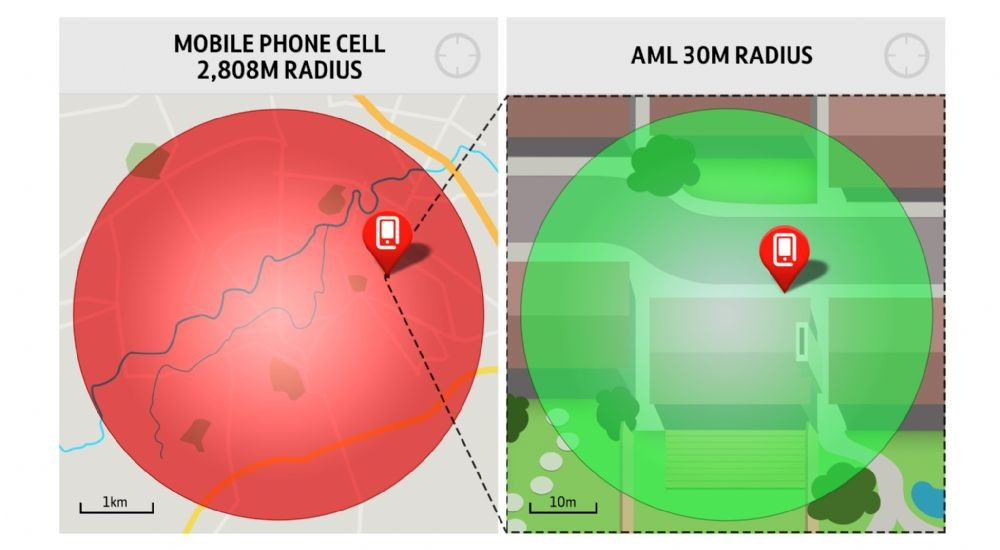
\includegraphics[scale=0.3,clip=true]{aml_radius}
  \caption{Localización sin AML vs con AML}
  \label{fig:aml_radius}
\end{figure}

Hace mucho tiempo que Android integró AML en todos sus dispositivos. En cambio, Apple integró AML en la actualización de iOS 11.3 en marzo de 2018 y funciona en un perímetro de menos de 100 metros en el 63% de los casos.

Como una consideración de desarrollo importante, AML se diseñó de modo que no interfiera con la llamada de emergencia por voz, por lo que si esta solución se replica en otros países de la Unión Europea, los desarrolladores deben confirmar que tanto el teléfono como la red móvil pueden admitir el establecimiento de ubicación GNSS o Wifi y la transmisión de SMS al PSAP a través de la red GSM durante una llamada de voz de emergencia estándar.

\subsubsection{Funcionamiento de AML}

Un teléfono móvil de hoy en día habilitado con AML reconoce cuando se realiza una llamada de emergencia y, si en este instante no está activado, activa el GNSS del dispositivo para recopilar la información de ubicación del usuario que llama. El teléfono luego envía un SMS (Short Message Service) automático a los servicios de emergencia (o PSAPs) con la ubicación actual de donde se encuentra el ciudadano, antes de volver a desactivar el GNSS.

SMS ofrece la mejor cobertura geográfica, especialmente en áreas remotas, y además, los SMS de emergencia generalmente no se cobran. El servicio también puede usar Wi-Fi, dependiendo de cuál sea mejor en ese momento dado.

\subsubsection{Beneficios de AML}

Según EENA, AML es 4.000 veces más preciso que la localización GSM tradicional, con un total del 85\% de las llamadas localizadas dentro de un radio de menos de 50 metros, mientras que con la localización mediante la red móvil, el radio puede tener varios kilómetros.

Las ventajas más llamativas de AML son:

\begin{itemize}
  \item Una vez implementado, el usuario no tiene que descargar ninguna app o realizar alguna acción adicional, sino que todo se hace de forma automática.
  \item El sistema ya acumula bastantes casos de éxito.
  \item La solución no ignora la información de Cell-ID que ya existía, sino que la complementa con información de GNSS o información de Wifi tomada del teléfono.
  \item Las redes móviles o los proveedores de dispositivos móviles no necesitaron una inversión significativa.
\end{itemize}

Pero AML todavía tiene algunas limitaciones, la principal es que no se ha extendido de forma global. El sistema ya funcionaba desde el 2016 en Reino Unido, Lituania, Austria y en Estonia, mientras que en otros países de la Unión Europea esperan desplegarlo o en están en fase de prueba.

\subsubsection{Android ELS}

Android incluye AML, desde la versión Gingerbread OS en adelante, a través del Servicio de Ubicación de Emergencia (ELS, por sus siglas en inglés, Emergency Location Service). ELS fue anunciada por Google en Julio de 2016 y ha sido una de las noticias más importantes de la industria en los últimos años.

\begin{figure}[htp!]
  \centering
  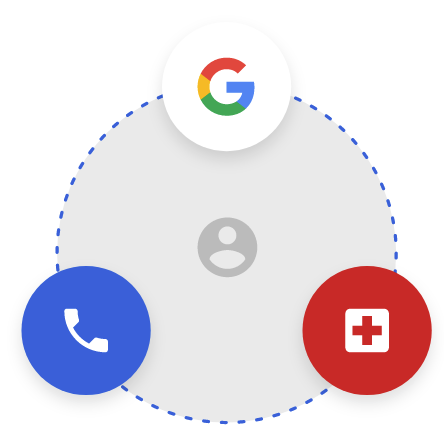
\includegraphics[scale=0.3,clip=true]{els_integration}
  \caption{Infraestructura de ELS}
  \label{fig:els_integration}
\end{figure}

Android ELS ayuda a los operadores de redes móviles, a los proveedores de infraestructura de emergencia y a los gobiernos a proporcionar información de ubicación más precisa a los PSAPs durante una emergencia. Cuando los servicios de emergencia reciben una llamada, deben conocer la ubicación de la persona que llama para enviar ayuda y salvar vidas.

Android ELS es compatible con más del 99\% de los dispositivos Android existentes (versión 4.0 y posteriores) a través de Google Play Services. Este servicio está disponible hoy en día y continúan interactuando activamente con los países y socios para hacer que ELS esté más disponible.

\subsection{NG112}

Actualmente, los servicios de emergencia solo son accesibles mediante llamadas telefónicas de voz, por lo que, tienen que cambiar su tecnología para ser parte del futuro; es decir, tener más en cuenta las comunicaciones basadas en Internet.

NG112 (Next Generation 112), un proyecto de EENA, busca la integración de las nuevas tecnologías en los servicios de emergencias, para recibir no solo voz, sino también información de ubicación, texto en tiempo real, ficheros multimedia, videollamadas y otra información relevante.

\begin{figure}[htp!]
  \centering
  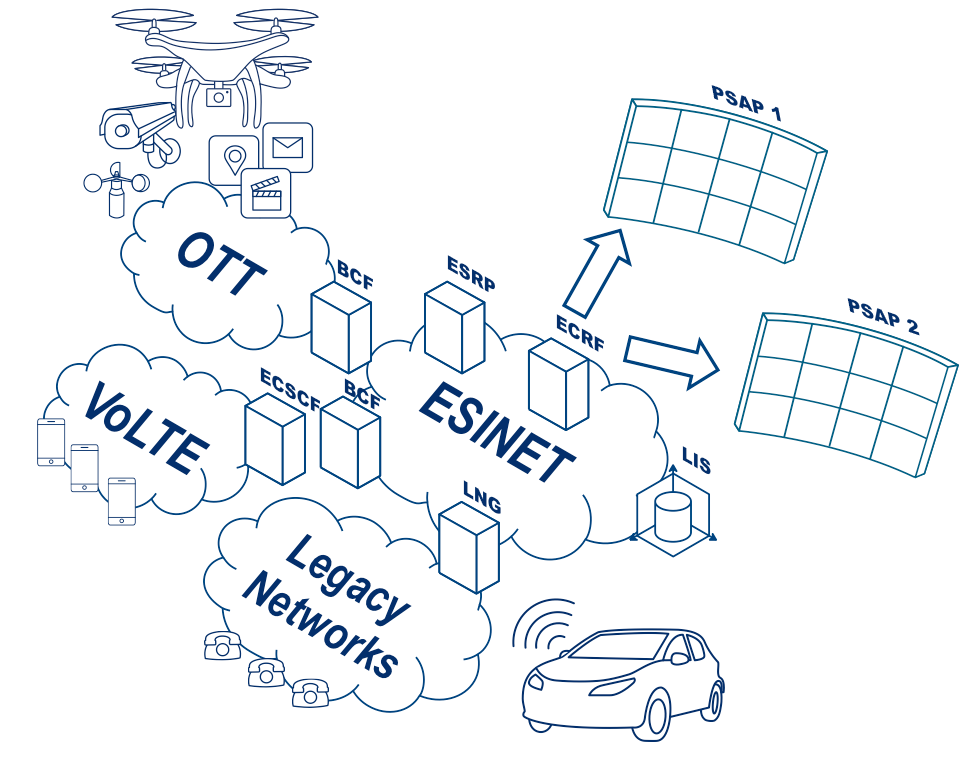
\includegraphics[scale=0.3,clip=true]{ng112_landscape}
  \caption{Panorama de NG112}
  \label{fig:ng112_landscape}
\end{figure}

Una de las razones, por las que desarrolló NG112, fue que los ciudadanos usan comunicaciones basadas en IP todos los días y quieren comunicarse con los servicios de emergencia utilizando estos métodos.

\subsubsection{Beneficios de NG112}

En contraposición a las limitaciones del modelo actual de 112, NG112 ofrece algunas ventajas:

\begin{itemize}
  \item Una infraestructura basada en el protocolo IP que implementa estándares abiertos y asegura interoperabilidad entre fronteras, agencias y proveedores.
  \item Métodos sólidos de adquisición y representación de información de localización con independencia del tipo de red.
  \item Permite al ciudadano acceder a los servicios de emergencia desde cualquier parte, y desde cualquier dispositivo, usando distintos tipos de medios (texto, voz o video) y aplicaciones.
  \item Nuevas funciones de mapeado y enrutamiento de llamadas que reemplazan los tradicionales códigos de área.
\end{itemize}

\subsection{PEMEA}

EENA empezó en 2016 a desarrollar un proyecto que busca que las apps que conectan a los ciudadanos con los servicios de emergencia deben funcionar por completo en cualquier lugar de la Unión Europea. Para lograr esto, las apps deben estar interconectadas de manera estandarizada. No se trata de crear una aplicación única, sino que múltiples aplicaciones móviles sean capaces de funcionar allá de donde estén.

EENA, junto con la empresa francesa Deveryware y la empresa italiana Beta 80, presentó a finales del mes de abril de 2018, el proyecto PEMEA (Pan-European Mobile Emergency App). PEMEA es un estándar ETSI, desarrollado bajo el proyecto H2020 NEXES, que busca la interconexión de apps de emergencias.

\begin{figure}[htp!]
  \centering
  
\includegraphics[scale=0.05,clip=true]{pemea_logo}
  \caption{Logo de PEMEA}
  \label{fig:pemea_logo}
\end{figure}

El objetivo de PEMEA es que una persona que llama por una emergencia pueda usar cualquier app de emergencias en cualquier lugar de Europa. Permitiendo a cualquier PSAP recibir información vital de la persona que llama, como idiomas o discapacidades, y una ubicación precisa para una respuesta de emergencia más rápida y efectiva.

Además, PEMEA define roles y responsabilidades así como formatos de intercambio de datos y un modelo general de seguridad de manera que los PSAPs puedan asegurarse de la veracidad de la información que les está siendo facilitada a través de la app, y a su vez los usuarios de la app pueden estar seguros de que la información que facilitan no está siendo usada indebidamente.

PEMEA se lanzó oficialmente el 11 de septiembre de 2018 en Madrid (España). De hecho, el beneficio para España es doble, ya que los usuarios no se verán obligados, como hasta ahora, a descargar diferentes apps de emergencias cuando viajan de una Comunidad Autónoma a otra dentro del propio país.

\subsubsection{Cómo funciona PEMEA}

La arquitectura PEMEA lleva a cabo los siguientes pasos a la hora de atender una llamada al 112:

\begin{enumerate}
  \item El usuario de la app de emergencias llama al 112.
  \item El AP (Application Provider) autentica al usuario, formatea los datos de la llamada antes de enviarlos al PSP (PSAP Service Provider).
  \item El PSP recupera información vital del usuario a partir de fuentes de confianza y los proporciona al PSAP.
  \item Si el usuario está en itinerancia, los datos se envían al ASP (Aggregating Service Provider) para fines de enrutamiento.
  \item El ASP proporciona enrutamiento de los datos para el PSP o PSAP más adecuado, o envía un error.
  \item Finalmente, el PSAP obtiene la información enviada y el usuario recibe la ayuda necesaria.
\end{enumerate}

\begin{figure}[htp!]
  \centering
  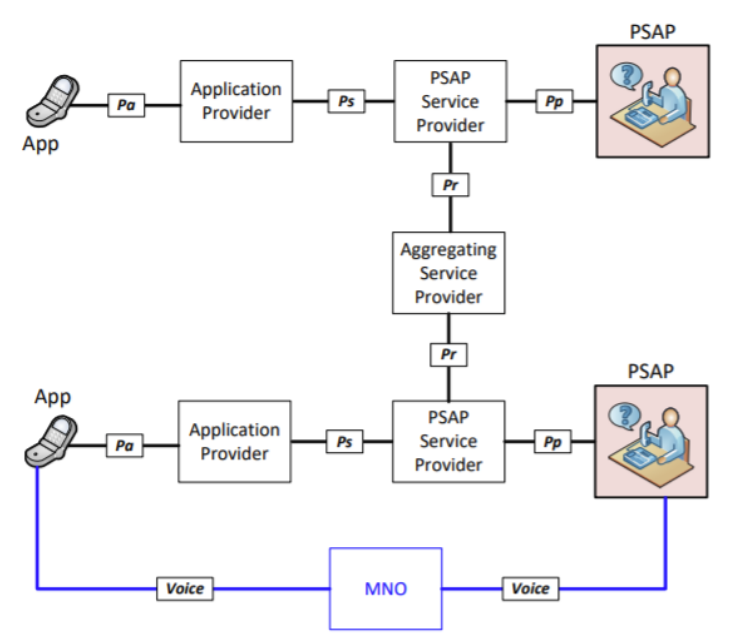
\includegraphics[scale=0.3,clip=true]{pemea_network}
  \caption{Arquitectura de PEMEA}
  \label{fig:pemea_network}
\end{figure}

\section{Apps de emergencias}

En un principio, la razón de añadir las apps de emergencias fue el uso de las capacidades de localización de alta precisión que incluyen los teléfonos móviles de hoy en día, para que dicha información pudiese ser enviada a los PSAPs.

Una app de emergencias puede ser muy útil si ocurre una emergencia y hace falta pedir ayuda. Algunas ya existentes permiten enviar de forma automática la localización a las unidades de atención de llamadas e incluso mandar fotografías para agilizar una primera intervención si es necesario. Pero los sistemas de comunicación con los centros de gestión de las llamadas al 112 no han evolucionado con la misma rapidez que la tecnología en tiempo real.

Aunque actualmente existen cientos de apps de emergencias, éstas no están integradas entre sí. Un viajero está obligado a descargarse la app que usan en la ciudad de destino, porque el centro de emergencias de esta ciudad no está habilitado para recibir esa solicitud.

\subsection{My112}

My112 es una app con la que podemos comunicarnos con el servicio de emergencias de ciertas comunidades autónomas de España. La app está disponible tanto en Android como en iOS y, por supuesto, de forma gratuita y sin anuncios. Es sencillo de usar: antes de llamar al 112 para cualquier emergencia, usamos la app para enviar nuestra ubicación actual, incluso si queremos, como información adicional, enviar también fotografías de lo que sucede. De este modo, enviamos mayor información de la emergencia a los PSAPs.

\begin{figure}[htp!]
  \centering
  
\includegraphics[scale=0.2,clip=true]{my112_logo}
  \caption{Logo de My112}
  \label{fig:my112_logo}
\end{figure}

My112 no está disponible en toda Europa, ni siquiera en toda España. Sólo funciona si la utilizamos en determinadas comunidades autónomas. Actualmente, My112 es compatible con los centros 112 de Madrid, Castilla y León, Islas Baleares, Cataluña, Cantabria y Melilla.

En realidad, la app no está desarrollada ni por el organismo que regula el 112 ni por ninguna entidad oficial, sino por Telefónica. Telefónica ha trabajado en coordinación con los centros de Emergencias 112 de las distintas comunidades.

\subsubsection{Avisos de emergencias en tiempo real}

My112 recibe avisos de emergencias en tiempo real cercanas a tu posición e información actualizada de las mismas en el momento de producirse. Cuando se produzca un aviso de emergencia en la zona donde te encuentres, recibirás una notificación con información asociada.

Estos avisos, para evitar la saturación, sólo se reciben si la persona se encuentra en la “zona cercana”. Los servicios de emergencia seleccionan un área en un mapa desde el panel de administración y todos los que estén dentro recibirán las alertas enviadas a ese grupo.

Pulsando sobre un aviso, se accede a la vista del mapa donde se puede observar geográficamente el área afectada por el aviso, nuestra posición con respecto al mismo y el texto del aviso lanzado desde el Centro 112.

En caso de no disponer de datos la aplicación enviará nuestra posición al 112 mediante un mensaje de texto SMS.

\section{Apps de mensajería instantánea}

Las apps de mensajería instantánea son el motivo de que muchos usuarios deciden dar el salto a los smartphones, ya que la posibilidad de enviar mensajes sin coste adicional resulta muy atractivo. Casi todo el mundo usa las apps de mensajería instantánea como principal medio de comunicación.

Hoy por hoy, WhatsApp es el rey indiscutible, sobre todo en España donde tiene una cuota de mercado realmente alta, dejando muy poco espacio para otros competidores. Pero a pesar de todo, si por cualquier motivo no os gusta WhatsApp existen muchas alternativas de calidad para utilizar la mensajería instantánea.

Todas parten sobre la misma base, chat de texto, voz e incluso videollamada, y luego tienen sus particularidades, interfaces de usuario muy distintas, una base de usuarios mayor o menor, y diferentes herramientas enfocadas a la seguridad o la privacidad.

\subsection{Skype}

Skype es el cliente de mensajería instantánea de Microsoft, que además se puede usar para comunicarse a través de voz y vídeo. Al ser multiplataforma, está disponible en Windows, Mac y Linux, así como en aplicaciones para tablets y smartphones.

\begin{figure}[htp!]
  \centering
  
\includegraphics[scale=0.2,clip=true]{skype_logo}
  \caption{Logo de Skype}
  \label{fig:skype_logo}
\end{figure}

Skype fundamentalmente lo asociamos con las videoconferencias, donde podemos comunicarnos simultáneamente con hasta 10 usuarios.  La posibilidad de llamadas de voz a través de Skype, incluso a teléfonos convencionales si tenemos créditos o estamos en un plan de pago hacen que sea una opción muy atractiva para tener instalada en el teléfono móvil.

Su apuesta por Skype Qik para compartir mensajes de vídeo entre amigos, es una opción interesante con la que trata de ganar terreno entre los usuarios.

\subsection{Facebook Messenger}

Facebook Chat, lanzada en 2008 por Facebook, fue la punta de lanza que renovó al mundo de la mensajería instantánea. En 2011 dio el salto definitivo en las apps con el lanzamiento de Facebook Messenger. Ahora no solo permite compartir archivos, sino también mensajes de voz, llamadas y videollamadas entre otras características como las reacciones ante las imágenes que recibimos de otros usuarios.

\begin{figure}[htp!]
  \centering
  
\includegraphics[scale=0.2,clip=true]{facebook_logo}
  \caption{Logo de Facebook Messenger}
  \label{fig:facebook_logo}
\end{figure}

Este es el cliente de mensajería instantánea de Facebook, que hoy en día se ofrece únicamente en dispositivos móviles (Android, iPhone, Windows Phone y BlackBerry) o mediante la página oficial de Facebook. Hace tiempo que se volvió independiente, y es uno de los más importantes en todo el mundo.

\subsection{WhatsApp}

El gran revulsivo en el ámbito de la mensajería instantánea, que ha llevado esta solución a ganar popularidad en los smartphones. Es una aplicación que ganó popularidad rápidamente y que fue adquirida por Facebook en 2014. Funciona en iOS, Android, BlackBerry, Windows Phone, Nokia, Symbian y Tizen. El nombre de usuario se define a través del número de teléfono, y ofrece soluciones para poder trabajar con él desde un PC.

\begin{figure}[htp!]
  \centering
  
\includegraphics[scale=0.05,clip=true]{whatsapp_logo}
  \caption{Logo de WhatsApp}
  \label{fig:whatsapp_logo}
\end{figure}

WhatsApp es para muchos la app de mensajería instantánea más importante del mundo. WhatsApp se lanzó en 2009 y hasta la fecha continúa dando sorpresas tras cada actualización. Mensajes instantáneos, llamadas de voz, videollamadas, notas de voz, compartir archivos y chats grupales son las características que hacen a WhatsApp la app líder en el mundo.

\section{Tecnologías de comunicación en tiempo real}

Uno de los grandes retos para la web fue permitir la comunicación humana a través de la voz y el vídeo: la comunicación en tiempo real o RTC (Real Time Communication). RTC debería ser tan natural en una aplicación web cómo la mensajería instantánea basada en texto. Sin ella, estábamos limitados en nuestra capacidad de innovar y desarrollar nuevas formas para que las personas interactúen \cite{webrtc3}.

No hay duda de que la VoIP (Voice over Internet Protocol) es una tecnología que está cambiando completamente el sistema de comunicación de las empresas. Convierte la voz en paquetes de datos para que trabaje a través de Internet y tu puedas disfrutar de una telefonía más efectiva con más prestaciones y mayor calidad \cite{webrtc2}.

Si ya has visto muchos sitios web de proveedores de VoIP, probablemente hayas encontrado un montón de acrónimos raros, como WebRTC o SIP.

\subsection{IM}

La mensajería instantánea se remonta a la década de los 60, cuando el MIT desarrolló una plataforma que permitía que hasta 30 usuarios pudieran iniciar sesión a la vez y enviarse mensajes entre ellos. El concepto creció en popularidad a medida que la tecnología avanzaba, y ahora damos por sentado la mensajería instantánea y la consideramos parte de nuestra vida cotidiana.

La mensajería instantánea o IM (Instant Messaging) es un servicio de comunicación en tiempo real que permite una conversación, casi siempre con alguien ya conocido, durante la cual un dispositivo móvil o sobremesa está conectado a otro con el fin de intercambiar texto. Utiliza el protocolo IP, siendo un servicio más que se proporciona a través de Internet.

La mensajería instantánea ha evolucionado desde el concepto de las salas de chat en línea públicas de los años 90 y 2000, y se ha vuelto bastante sofisticada y muy común. Algunas compañías usan este servicio como parte de sus herramientas de productividad y comunicación.

Con el auge de las redes sociales y servicios como Facebook y Twitter, así como el cambio a dispositivos móviles como teléfonos inteligentes y tablets, la mensajería instantánea ha perdurado y evolucionado.

La mensajería instantánea crece "de forma imparable" como primera forma de comunicación, imponiéndose incluso a la comunicación en persona. El uso de la mensajería instantánea es especialmente significativo entre los jóvenes.

Algunos productos de mensajería instantánea son básicos, que funcionan esencialmente como mensajes de texto. Otros sistemas de mensajería instantánea ofrecen opciones avanzadas que le permiten hacer más que enviar mensajes de texto, como la posibilidad de compartir fotos, enviar y recibir archivos.

\subsubsection{Cómo funciona la mensajería instantánea}

La mensajería instantánea se basa en pequeños programas, conocidos como clientes, que dos personas independientes instalan, y esos programas se conectan para transmitir mensajes escritos entre sí.

Para que dos personas se puedan comunicar usando IM, cada uno debe tener instalado uno de estos programas, que se conectan entre sí para enviar mutuamente mensajes de texto u otro contenido multimedia.

La forma en que la comunicación ocurre se puede describir de la siguiente manera:

\begin{enumerate}
  \item Usando un cliente de IM, tecleas tu usuario y contraseña.
  \item El cliente se conecta a un servidor usando Internet y algún protocolo de comunicación, que es usualmente específico para el servicio que estés usando.
  \item El servidor verifica tu identidad y crea un registro temporal de tu conexión y los contactos que tienes en tu lista.
  \item El servidor verifica quiénes de tu lista de contactos está en línea y le da esa información al cliente, que a su vez hará lo necesario para mostrarlos. Asimismo, les indicará a los clientes de esos contactos que tú estás en línea.
  \item Seleccionas una persona a la que le enviaras un mensaje. Tecleas tu mensaje y lo envías. En este momento tu software cliente sabe a qué IP y puerto enviar el mensaje y el cliente de tu contacto le muestra el mensaje.
  \item La otra persona te escribe un mensaje, repitiendo el proceso y así llevando a cabo una conversación.
  \item Cuando cierras tu cliente, el servidor se da cuenta de que estás fuera de línea y le comunica a los clientes de tus contactos que ya no estás en línea. El servidor destruye el registro temporal que se había creado cuando te conectaste.
\end{enumerate}

\subsection{SIP}

SIP proviene de Session Initiation Protocol y es la tecnología más utilizada por los proveedores de telefonía IP. Es la razón de la revolución de los sistemas de comunicaciones. Ha mejorado la telefonía tradicional añadiendo muchas funcionalidades útiles para las empresas, como la mensajería instantánea o las conferencias telefónicas \cite{webrtc2}.

El protocolo SIP, desarrollado por el grupo MMUSIC, te permite recibir o realizar llamadas de voz a través de Internet, utilizando para ello terminales IP especiales, o bien de software (softphones) o de hardware \cite{webrtc1}.

\subsubsection{Beneficios y riesgos de utilizar SIP}

Las ventajas de utilizar SIP son:

\begin{itemize}
  \item \textbf{Buena calidad de llamada}. La calidad de llamada en el protocolo SIP, aunque siempre ha sido cuestionada, podemos decir que es buena, siempre y cuando cuentes con una buena conexión de Internet. Si recibes por datos o en una zona con mala cobertura de Internet notarás como desciende mucho la calidad.
  \item \textbf{Experiencia}. El protocolo SIP está más que testeado ya que tiene muchos años de vida.
  \item \textbf{Gran abanico de posibilidades}. Es mucho más ofertado por las empresas de telefonía por lo que tienes más donde elegir.
\end{itemize}

Las desventajas de utilizar SIP son:

\begin{itemize}
  \item \textbf{Poca versatilidad}. En cuanto a la flexibilidad y versatilidad del servicio, el protocolo SIP pierde claramente ya que para recibir o emitir llamadas tienes que hacerlo a través de terminales IP o softphones, por lo que estás más limitado.
  \item \textbf{Relación calidad/precio}. La relación calidad/precio en este caso no es tan buena ya que normalmente tienes que efectuar una gran inversión en equipos para poder utilizarlo, además las empresas que lo ofrecen suelen ser algo más caras.
  \item \textbf{Alta Inversión inicial}. El protocolo SIP necesita terminales especiales para funcionar. Tienes varias opciones, o bien utilizar softphones que podrás instalar en tu móvil o bien adquirir terminales IP que requieren una gran inversión inicial.
\end{itemize}

\subsection{WebRTC}

La tecnología WebRTC es un software de código abierto desarrollado por Google y que te permite realizar o recibir llamadas de voz a través del navegador o de una app \cite{webrtc1}. Transporta la voz utilizando las aplicaciones del navegador, por lo que, a diferencia del SIP, no necesitarás ningún dispositivo adicional. Puedes usarlo en tu smartphone o tablet descargando una aplicación, o en tu PC usando un par de auriculares \cite{webrtc2}.

\begin{figure}[htp!]
  \centering
  
\includegraphics[scale=0.3,clip=true]{webrtc_logo}
  \caption{Logo de WebRTC}
  \label{fig:webrtc_logo}
\end{figure}

WebRTC significa Web Real Time Communication y es una tecnología de estándares abiertos que permite comunicaciones en tiempo real nativamente desde un navegador web, sin la necesidad de descargas adicionales o plugins, gracias a una API de JavaScript y el códec VP8. \cite{webrtc3}

WebRTC se utiliza en varias aplicaciones como WhatsApp, Facebook Messenger, appear.in y plataformas como TokBox \cite{webrtc3}.

\subsubsection{Beneficios y riesgos de utilizar WebRTC}

Las ventajas de utilizar WebRTC son:

\begin{itemize}
  \item \textbf{Completa Versatilidad}. Una de las mayores ventajas del protocolo WebRTC es la versatilidad que ofrece. Al poder utilizarse en cualquier dispositivo sin necesidad de disponer de un terminal especial, puedes utilizarlo en cualquier lugar del mundo siempre que cuentes con un dispositivo con conexión a Internet.
  \item \textbf{Excelente calidad de llamada}. El protocolo WebRTC es capaz de modular la voz dependiendo del nivel de datos y la cobertura de la conexión a Internet de la que dispongas en cada momento para que la calidad de la voz siempre sea buena \cite{webrtc1}.
  \item \textbf{Relación calidad/precio}. Las empresas que ofrecen WebRTC normalmente ofertan soluciones más económicas que sus competidoras las que ofrecen soluciones SIP y con resultados más competitivos.
  \item \textbf{Sin inversión inicial}. Si lo utilizas desde tu ordenador, simplemente tendrás que adquirir unos auriculares con micrófono y si lo utilizas desde el móvil, ni eso. Por lo que te ahorrarás ese desembolso inicial en terminales especiales que suele ser bastante elevado.
  \item \textbf{Interfaz online}. Al ser un protocolo que se utiliza a través del navegador, contarás con una interfaz online mucho más visual que en un terminal IP.
\end{itemize}

\section{Estrategias de comunicación en tiempo real}

Para muchos, lo primero que se nos viene a la mente cuando hablamos de aplicaciones web en tiempo real, es el uso de WebSocket, sin embargo, como verás a continuación, la respuesta a la implementación de comunicación en tiempo real, no siempre deben ser usando WebSocket.

A continuación vienen algunas de las estrategias que los desarrolladores web han implementado para poder establecer una comunicación constante con el servidor, que les permita mantener la información actualizada, justo cuando sucede.

\subsection{Polling}

La más simple de todas las formas es el pooling. Es muy simple, para saber si algo pasa, tenemos que preguntar constantemente. La estrategia del pooling consiste en consultar al servidor en un periodo constante de tiempo, usualmente muy pequeño, digamos cada 3 segundos. En términos más técnicos, implementar pooling significa realizar peticiones al servidor cada par de segundos, para consultar información nueva.

Las ventajas del pooling son:

\begin{itemize}
  \item Es extremadamente simple realizar peticiones constantes cada cierto periodo de tiempo.
  \item No requiere de tecnologías especiales más que AJAX, para poder hacer las consultas.
  \item Muy fácil de implementar, sólo colocas tus consultas en un intervalo y listo.
\end{itemize}

Así como la implementación es muy simple, las desventajas de usar pooling son también muy claras:

\begin{itemize}
  \item Sobrecargas al servidor, es muy probable que muchas de las peticiones reciban como respuesta nada, en caso de que no haya información nueva que comunicar, sin embargo, las peticiones siguen ejecutándose y el servidor tiene que responderlas.
  \item Pequeña latencia. Si tu aplicación es de respuesta crítica, considera que con el pooling siempre habrá un ligero retraso entre el momento en el que la información se produce y el momento en el cliente se entera, si por ejemplo, mandas una petición cada 10 segundos, este será el tiempo máximo en que la información podría llegar retrasada.
\end{itemize}

\subsection{Long polling}

Al notar que muchas de las respuestas que se reciben las peticiones de una implementación con pooling, son respuestas vacías porque el servidor no tiene nada nuevo que comunicar, se introdujo una mejora a dicha estrategia, la llamaron long pooling.

El flujo de una implementación con long pooling es la siguiente:

\begin{enumerate}
  \item El cliente envía una petición HTTP al servidor consultando información nueva.
  \item El servidor tiene dos opciones:
  \begin{enumerate}
    \item Si existe información nueva que reportar, la envía inmediatamente.
    \item Si no existe información nueva que reportar, mantiene esta conexión HTTP en espera y abierta, hasta que exista algo que reportar, entonces envía la información al cliente y cierra dicha conexión.
  \end{enumerate}
  \item El cliente recibe respuesta de su mensaje con datos nuevos, ya sea tan pronto como la envió o luego de haber esperado por bastante tiempo a que hubiera algo nuevo que reportar.
  \item El cliente manda una nueva petición hasta que la anterior fue contestada, así, esta nueva recibirá respuesta hasta que haya nuevos datos.
\end{enumerate}

\begin{figure}[htp!]
  \centering
  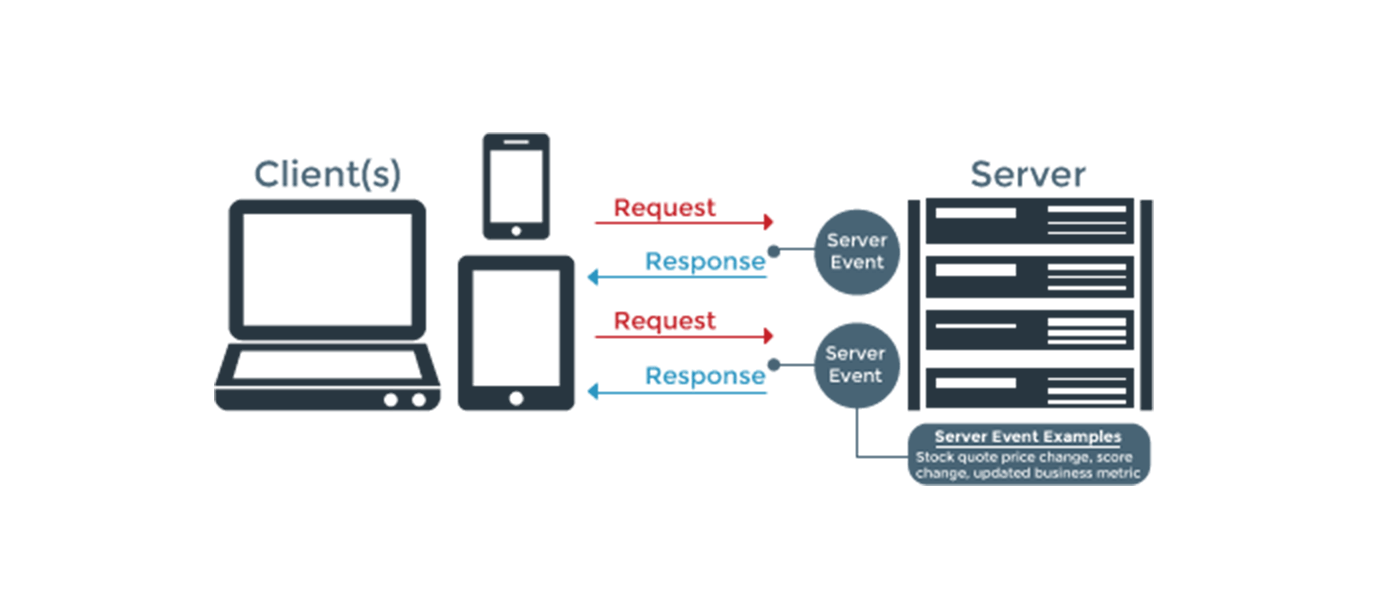
\includegraphics[scale=0.3,clip=true]{long_polling}
  \caption{Funcionamiento de Long polling}
  \label{fig:long_polling}
\end{figure}

La clara diferencia entre el long pooling y el pooling es que en esta mejora de la estrategia anterior, no se envía peticiones constantes, más bien se envía una inicial y las siguientes sólo se envían hasta que hubo una respuesta previa, con datos actualizados. Esto reduce drásticamente la cantidad de peticiones que enviamos hacia el servidor.

Las ventajas del long pooling son las siguientes:

\begin{itemize}
  \item Todas las del pooling, a final de cuentas es casi la misma metodología.
  \item Menos peticiones que el pooling, por lo tanto, un servidor con menos carga y más eficiente.
  \item Mejora significativa en qué tan rápido recibimos los datos nuevos, ya que para cuando estos se crean, ya hay una conexión esperando para que se envíen al cliente.
\end{itemize}

Las desventajas son más difíciles de identificar, pero sucede:

\begin{itemize}
  \item Seguimos realizando y abriendo peticiones HTTP, aún cuando estas quizás nunca reciban respuesta.
  \item Algunos servidores no permiten que las conexiones HTTP permanezcan abiertas por mucho tiempo, por lo que cada que se cierran, debemos crear peticiones nuevas, aumentando la carga del servidor.
\end{itemize}

\subsection{WebSocket}

En 2010, justo en la cúspide de la popularidad del término HTML5, se introdujo al navegador la habilidad de establecer conexión a dos vías, directamente con el servidor, el protocolo WebSocket.

\begin{figure}[htp!]
  \centering
  
\includegraphics[scale=0.2,clip=true]{websocket_logo}
  \caption{Logo de WebSocket}
  \label{fig:websocket_logo}
\end{figure}

WebSocket es un protocolo que permite crear un canal de comunicación bidireccional (full-duplex) sobre una única conexión TCP. Está pensado para ser implementado en navegadores y servidores web, aunque no hay ningún impedimento a la hora de implementarlo en cualquier otro tipo de aplicación que siga el modelo cliente/servidor.

Es el mismo concepto de los clásicos sockets de UNIX, pero en la Web, y con la idea de facilitar la transferencia de datos en tiempo real entre un cliente y un servidor web. Siendo una comunicación bidireccional, el servidor web puede enviar la información directamente al cliente durante la conexión.

Las comunicaciones se realizan a través de los mismos puertos que utiliza HTTP con el fin de ofrecer compatibilidad con el software HTTP del lado del servidor ya existente. Es decir, cuando el protocolo trabaja directamente sobre TCP utiliza el puerto 80 y cuando lo hace sobre TLS utiliza el 443. No obstante, WebSocket es un protocolo independiente.

\subsubsection{Funcionamiento básico}

El protocolo se divide en dos partes: la negociación y la transferencia de datos. Como este coexiste con HTTP, la primera comunicación debe realizarse necesariamente a través de una petición HTTP. Por ello, la negociación de apertura comienza con una petición upgrade por parte del cliente, que tiene el siguiente aspecto:

\begin{figure}[htp!]
  \centering
  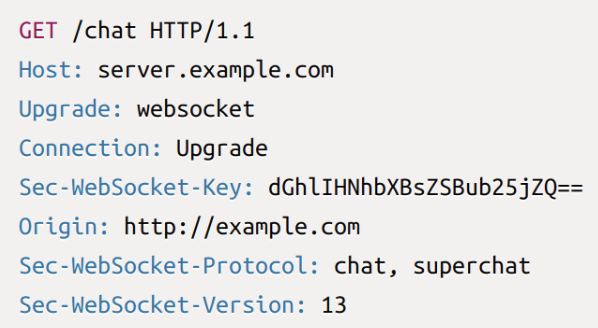
\includegraphics[scale=0.4,clip=true]{websocket_1}
  \caption{Pentición Upgrade del cliente}
  \label{fig:websocket_1}
\end{figure}

Cabe destacar que la elección del método GET es una decisión arbitraria tomada por los autores del borrador que finalmente quedó plasmada en el RFC. Aun así, es el único método que contempla el estándar y, por tanto, el único que se debe utilizar. Por su parte, si todo va bien, el servidor responde con un estado 101 (switching protocols), que tiene el aspecto que sigue:

\begin{figure}[htp!]
  \centering
  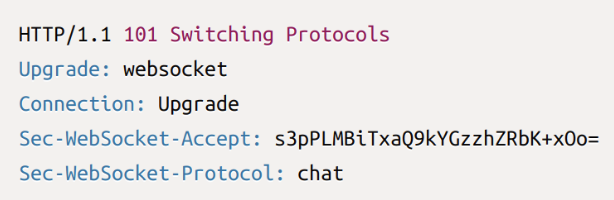
\includegraphics[scale=0.4,clip=true]{websocket_2}
  \caption{Respuesta de la petición Upgrade}
  \label{fig:websocket_2}
\end{figure}

En ambos casos, tanto en la petición como en la respuesta, se incluyen una serie de cabeceras: obligatorias de HTTP/1.1 (Host), necesarias para establecer la negociación (Upgrade, Connection y Sec-WebSocket-*) o por cuestiones relacionadas con modelo de seguridad escogido para el protocolo (Origin).

Una vez el cliente y el servidor han cumplido con su parte de la negociación, y únicamente si no ha ocurrido ningún error, comienza la transferencia de información. A partir de ese momento cada parte puede enviar información a placer sin depender de la otra, cosa imposible de hacer con HTTP, AJAX, las tecnologías push en general o técnicas más específicas como long polling.

\begin{figure}[htp!]
  \centering
  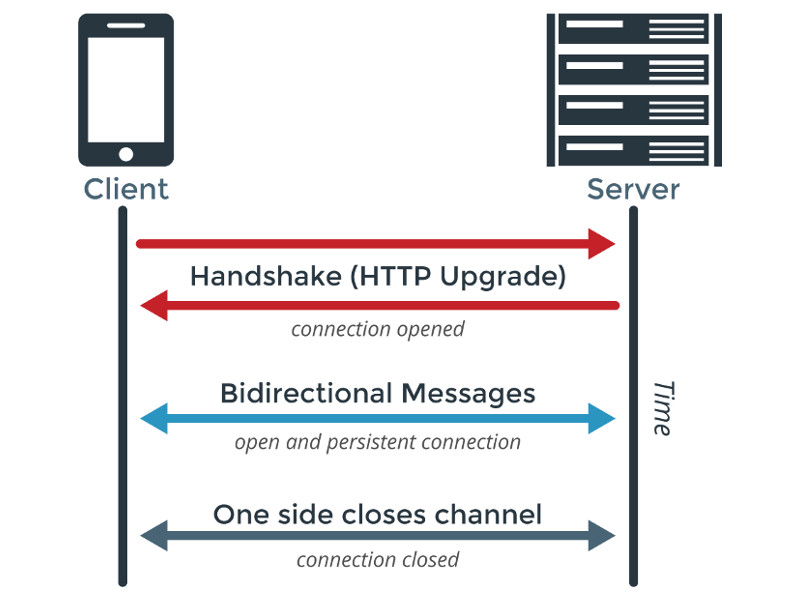
\includegraphics[scale=0.3,clip=true]{websocket}
  \caption{Funcionamiento de WebSocket}
  \label{fig:websocket}
\end{figure}

Por último, cuando una de las partes decide que ya no hay nada más que transmitir, es posible cerrar la conexión mediante una negociación de cierre. Esta se inicia enviando un mensaje de control específico, al cual el otro extremo responde con otro mensaje de control para confirmar que el cierre es acordado. La negociación de cierre está pensada para ir acompañada del cierre de la conexión TCP.

\subsection{SSE}

A diferencia de los WebSockets, los Server-Sent Events (SSE) son un canal de comunicación unidireccional donde los eventos fluyen del servidor a cliente únicamente. Los eventos enviados por el servidor permiten que los clientes del navegador reciban un stream de eventos a través de una conexión HTTP sin polling \cite{sse2}.

Un cliente se suscribe a un "stream" de un servidor y el servidor enviará mensajes, event-stream, al cliente hasta que el servidor o el cliente cierre el stream. Depende del servidor decidir cuándo y qué enviar al cliente, por ejemplo, tan pronto como cambian los datos.

\begin{figure}[htp!]
  \centering
  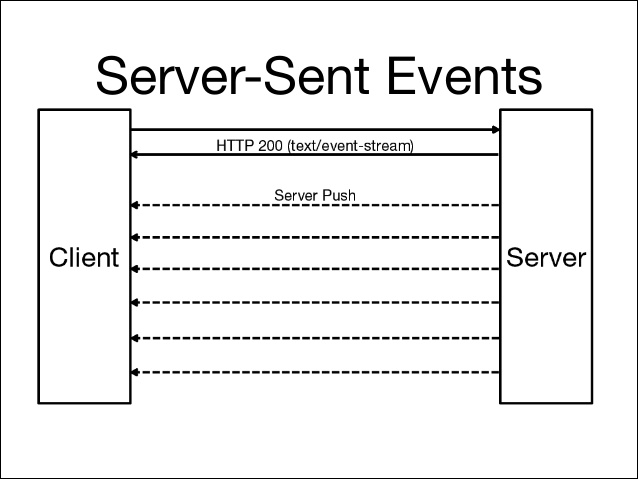
\includegraphics[scale=0.3,clip=true]{sse}
  \caption{Funcionamiento de SSE}
  \label{fig:sse}
\end{figure}

SSE es un estándar que describe cómo los servidores inicializan la transmisión de datos con el cliente una vez una conexión de cliente inicial se establece. Esta tecnología fue propuesta por el WHATWG (Web Hypertext Application Technology Working Group) y se implementó por primera vez en el navegador web Opera en el año 2006 \cite{sse1}.

También ofrece una API de JavaScript denominada EventSource implementada en la mayoría de los navegadores modernos como parte del estándar HTML5 de W3C. Hay polyfills disponibles para los navegadores que no son compatibles con la API de EventSource \cite{sse3}.

\section{Protocolos de mensajería instantánea}

En la actualidad existe una gran variedad de protocolos que son usados en la mensajería instantánea, algunos de ellos son propietarios y por tal motivo no ofrecen documentación ni dan acceso a sus fuentes, por otra parte, hay otros que son libres y están muy bien documentados a disposición de todos los usuarios.

Para poder mantener una comunicación a través de mensajería instantánea, es necesario hacer uso de un cliente que realice el servicio. En un primer momento cada servicio permitía conectarse únicamente con los usuarios que utilizaban ese mismo servicio. Más adelante veremos, que algunos protocolos hacen posible conectar varios servicios desde una misma cuenta.

Con respecto a la seguridad, por norma general, los protocolos no implementan (o habilitaban por defecto) el cifrado de las comunicaciones, transmitiendo éstas en texto claro y quedando expuestas a numerosos ataques como el robo de información, suplantación de identidad, alteración de la información transmitida, entre otros.

\subsection{MSNP}

MSNP (Mobile Status Notification Protocol) es el protocolo de mensajería instantánea de Microsoft. El cliente oficial de mensajería instantánea era Windows Live Messenger. A pesar de la popularidad de Windows Live Messenger, en 2013 cancelaron el servicio forzando a sus usuarios a utilizar en su lugar Skype.

A pesar de que el protocolo MSNP no es de código abierto, a través de técnicas de ingeniería inversa se ha podido conocer su funcionamiento. En la arquitectura del protocolo hay presentes tres tipos distintos de servidores utilizados para distintos procesos, siendo éstos 'Dispatch Server' (DS), 'Notification Server' (NS) y 'Switchboard Server' (SS).

\subsection{OSCAR}

OSCAR (Open System for Communication in Real-time) es el protocolo de mensajería instantánea de AOL. Este protocolo es implementado por los dos principales clientes de la compañía, AIM e ICQ. Al igual que ocurría con MSNP, OSCAR no es de código abierto pero también se ha podido acceder a una gran parte de su funcionamiento gracias a técnicas de ingeniería inversa.

Al igual que MSNP, la arquitectura detrás de OSCAR consta de varios servidores con distintas finalidades, siendo los principales el 'Authorization Server' (AS) y el 'Basic OSCAR Service Server' (BOSS).

Las conexiones con los servidores se realizan a través de distintos canales (frames). Gracias a estos canales es posible realizar comunicaciones paralelas sin necesidad de conectarse a múltiples servidores.

\subsection{YMSG}

El protocolo YMSG (Yahoo! Messenger) fue publicado en junio de 1999 y era similar a MSNP. Una de las novedades que introdujo fue su excelente integración con la Web. Al igual que ocurre con el resto de protocolos comentados, YMSG tampoco es de código abierto.

Con respecto a la arquitectura, se trata de un sistema cliente-servidor pero que, al contrario que en los protocolos MSNP y OSCAR, el cliente se conecta con un servidor aleatorio y a través de él realizará el resto de transmisiones (autenticación, acceso a la lista de contactos, comunicación con otro usuario, etcétera).

\subsection{XMPP}

La especificación base de Jabber, más tarde XMPP, surgió en 1998 por Jeremie Miller, conocido como el primero de carácter abierto y tomado como protocolo por la comunidad open source en 1999, donde ha ido creciendo y evolucionando hasta la actualidad.

XMPP (eXtensible Messaging and Presence Protocol) es un protocolo abierto y extensible, que establece una plataforma para el intercambio de datos en XML y que se utiliza principalmente en servicios de mensajería instantánea.

\begin{figure}[htp!]
  \centering
  
\includegraphics[scale=0.2,clip=true]{xmpp_logo}
  \caption{Logo de XMPP}
  \label{fig:xmpp_logo}
\end{figure}

Posee muchas implementaciones abiertas de servidores, clientes y librerías para las más diversas plataformas y lenguajes. Su funcionamiento topológico se basa en la clásica arquitectura cliente / servidor en la que no existen servidores centrales que gestionan el servicio sino que cualquier usuario puede crear su propio servidor XMPP.

Este protocolo es utilizado en aplicaciones y servicios conocidos como Google Talk, Tuenti, Facebook y WhatsApp (con algunas variaciones del mismo adaptadas al funcionamiento propio del servicio).

\section{Aplicaciones web}

Una aplicación web se basa en una arquitectura cliente/servidor, donde tanto el cliente (interfaz de usuario) como el servidor (servidor web) y el protocolo mediante el que se comunican (HTTP) están estandarizados y no han de ser creados por el desarrollador de aplicaciones.

\begin{figure}[htp!]
  \centering
  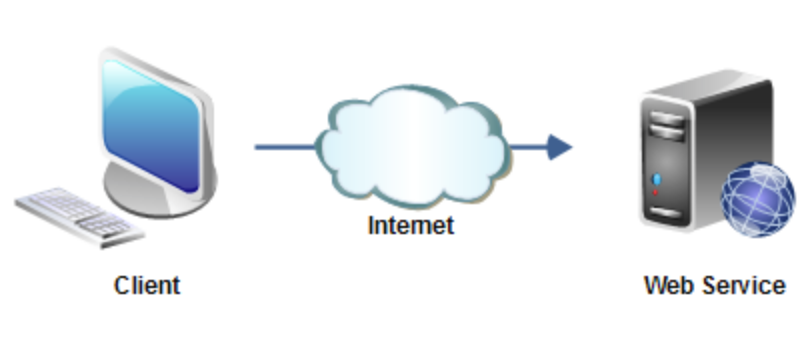
\includegraphics[scale=0.2,clip=true]{modelo_client_server}
  \caption{Arquitectura cliente/servidor}
  \label{fig:modelo_client_server}
\end{figure}

La arquitectura de una aplicación web suelen ajustarse a un modelo de tres capas. Este modelo supera las limitaciones de las arquitecturas ajustadas a un modelo de dos capas, introduciendo una capa intermedia (capa de proceso), entre la capa de presentación y  capa de datos. Cada capa es un proceso separado y bien definido corriendo en plataformas separadas.

Las capas que pueden identificarse en la arquitectura de una aplicación web son:

\begin{itemize}
  \item \textbf{Capa de presentación o cliente web}. El cliente web es un programa con el que interacciona el usuario para solicitar a un servidor web el envío de los recursos que desea obtener mediante HTTP. El cliente web recoge la información del usuario a través de una interfaz de usuario y la envía a la capa de proceso, después recibe los resultados de la capa de proceso y presenta los resultados al usuario.
  \item \textbf{Capa de proceso o servidor web}. El servidor web es un programa que está esperando permanentemente solicitudes de conexión, mediante el protocolo HTTP, por parte de la capa de presentación. En los sistemas Unix suele ser un demonio y en los sistemas Microsoft Windows un servicio. El servidor web recibe una petición por parte de la capa de presentación, éste interactúa con la capa de datos para realizar operaciones y envía los resultados procesados a la capa de presentación.
  \item \textbf{Capa de datos o servidor de base de datos}. El servidor de base de datos proporciona y almacena datos relevantes para la aplicación. Además, también puede proporcionar la lógica de negocio u otra información administrada por el servidor web.
\end{itemize}

\begin{figure}[htp!]
  \centering
  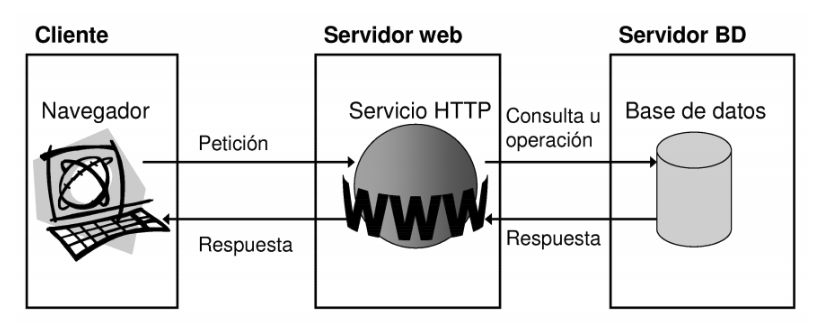
\includegraphics[scale=0.3,clip=true]{aplicacion_web}
  \caption{Arquitectura de una aplicación web}
  \label{fig:aplicacion_web}
\end{figure}

La interfaz de usuario no es requerida para comprender o comunicarse con el servidor de base de datos. La separación de roles en tres capas, hace más fácil reemplazar o modificar una capa sin afectar a las capas restantes.

\subsection{Servidor web}

Los servidores web son intrínsecos al funcionamiento de las aplicaciones web, lo que exige la necesidad de un mayor énfasis en la arquitectura del servidor web, incluida la capacidad física del servidor: almacenamiento, memoria, potencia de cómputo y rendimiento, además de los niveles de la aplicación. Esto podría estar en cualquier lugar, ya sea dentro del servidor, a través de la red o los sistemas operativos.

Los requisitos de una solución determinan el alcance de las arquitecturas de servidores web; por ejemplo, las soluciones pueden ser aplicaciones simples o de múltiples niveles.

Los diferentes tipos de arquitectura de servidor web incluyen:

\subsubsection{Java}

En virtud de ser un lenguaje de programación versátil, Java es popular en el entorno de desarrollo empresarial.

\begin{figure}[htp!]
  \centering
  
\includegraphics[scale=0.1,clip=true]{java_logo}
  \caption{Logo de Java}
  \label{fig:java_logo}
\end{figure}

Independientemente de la complejidad o la naturaleza de la aplicación, una arquitectura de un servidor web en Java es la plataforma preferida por los desarrolladores para crear soluciones y entregarlas según las expectativas.

Una de las ventajas distintivas de esta arquitectura es la capacidad de combinar y confiar en las herramientas nativas de Java y los frameworks para crear aplicaciones que abarcan todo el espectro, desde las aplicaciones más sencillas hasta las más complejas.

\begin{figure}[htp!]
  \centering
  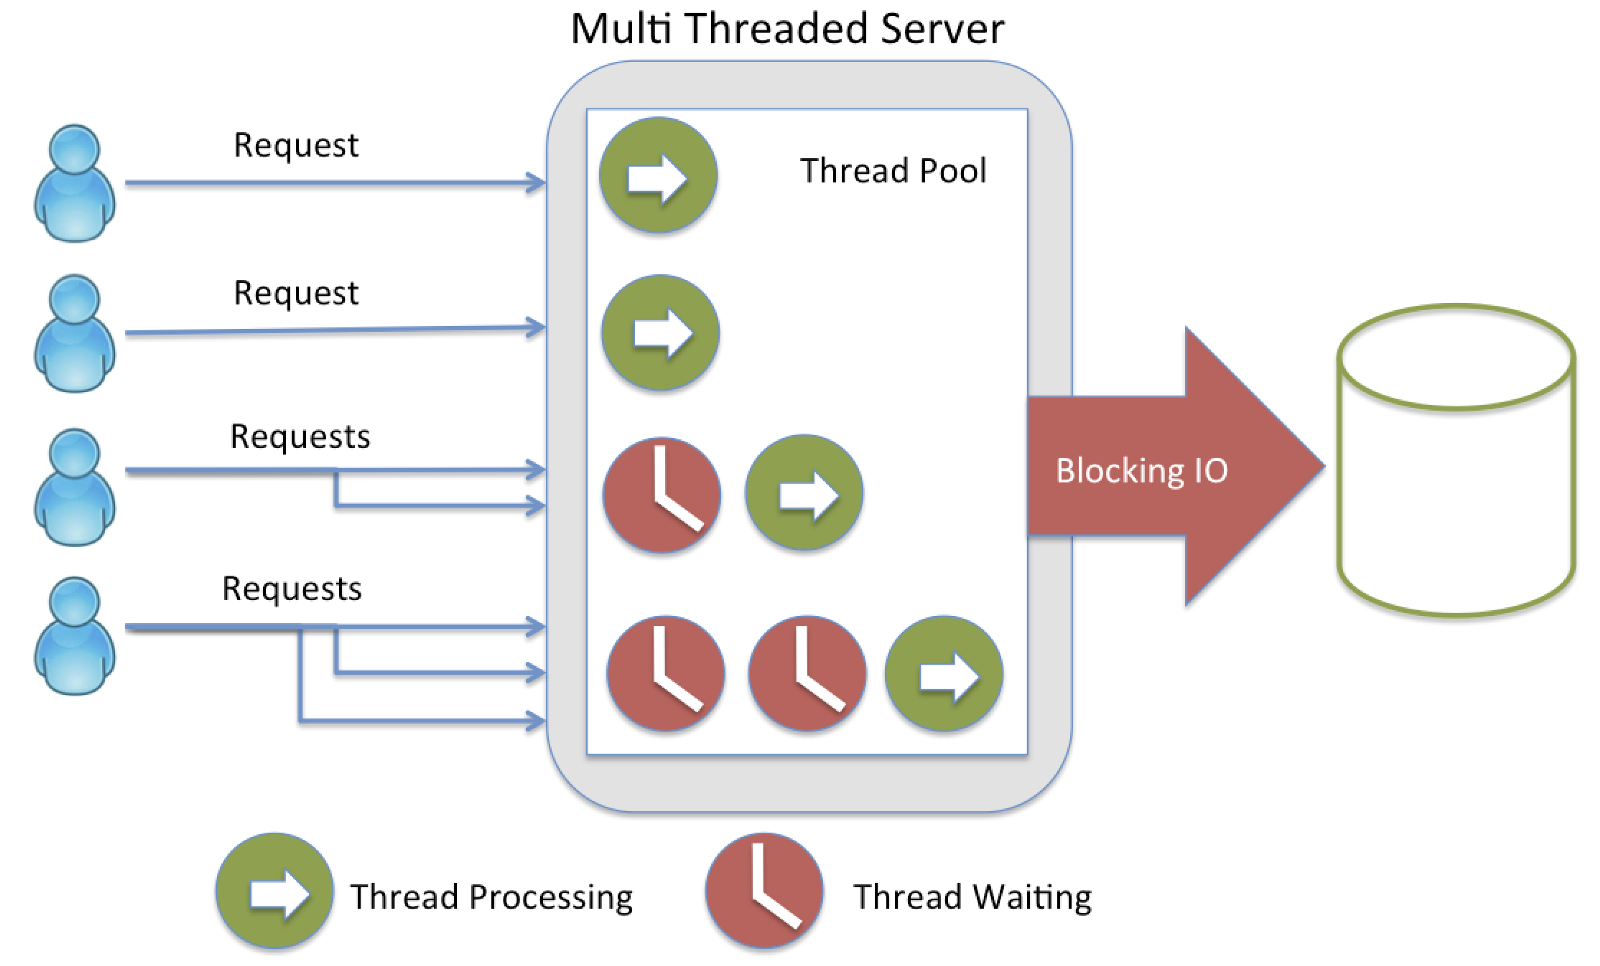
\includegraphics[scale=0.2,clip=true]{java_server}
  \caption{Arquitectura basada en Java}
  \label{fig:java_server}
\end{figure}

\subsubsection{Node.js}

Hace 24 años que Netscape creó JavaScript: un lenguaje de programación creado para manipular las páginas web mediante scripts dentro de su navegador web.

En 2008 Google lanza su navegador Chrome, junto con su motor de JavaScript V8. Un año después Ryan Dahl usaría V8 como base para crear Node.js y cambiar la forma en que se conocía JavaScript.

\begin{figure}[htp!]
  \centering
  
\includegraphics[scale=0.2,clip=true]{nodejs_logo}
  \caption{Logo de Node.js}
  \label{fig:nodejs_logo}
\end{figure}

Node.js es un entorno open source de desarrollo de software o programación con el objetivo de cubrir ciertas necesidades de los programadores a la hora de trabajar con Javascript en el lado del servidor.

Node.js utiliza un modelo de entrada/salida sin bloqueo controlado por eventos, de esta manera lo hace un entorno ligero y eficiente.

Su propuesta se basa en el tratamiento de conexiones de forma unificada a partir de un único hilo complementado con un bucle de eventos de tipo asíncrono. De este modo las peticiones que se vayan haciendo reciben un tratamiento en forma de eventos y pertenecen a este único bucle.

Este nuevo replanteamiento proporciona un lenguaje con la capacidad de gestionar una gran cantidad de solicitudes y conexiones con la máxima eficiencia.

\begin{figure}[htp!]
  \centering
  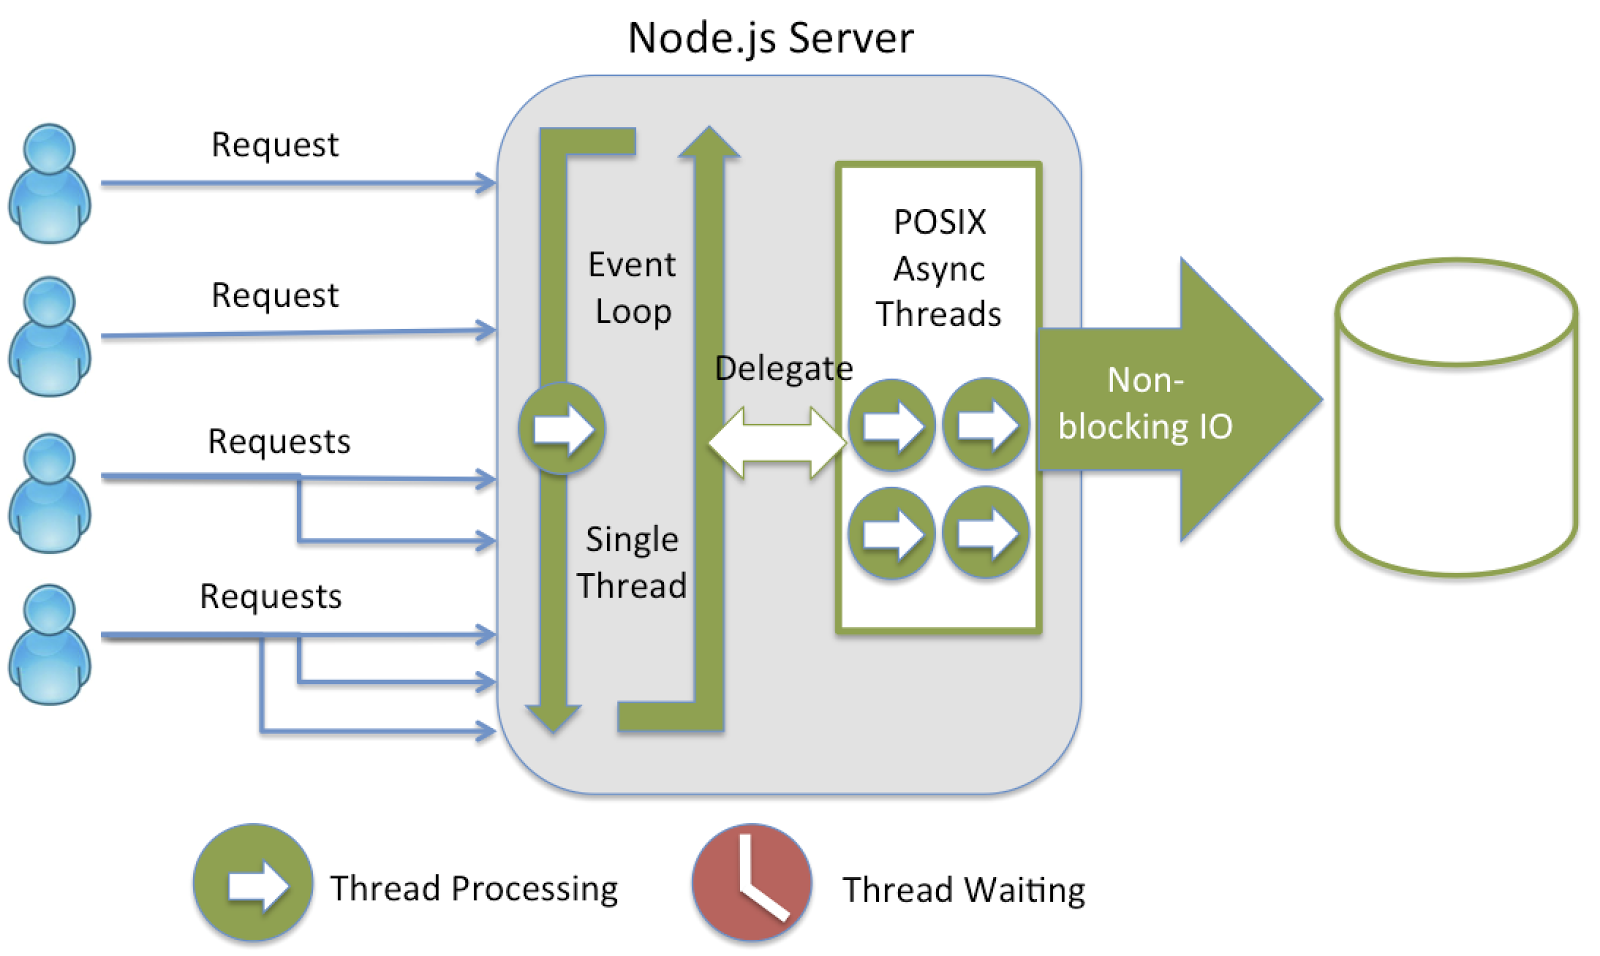
\includegraphics[scale=0.2,clip=true]{nodejs_server}
  \caption{Arquitectura basada en Node.js}
  \label{fig:nodejs_server}
\end{figure}

\subsection{Servidor de base de datos}

Los servidores de base de datos surgen en la década de los 80 con motivo de la necesidad de las empresas de manejar grandes y complejos volúmenes de datos, al tiempo que requieren compartir la información con un conjunto de clientes de una manera segura y debe proporcionar servicios de forma global y, en la medida de lo posible, independientemente de la plataforma.

Un servidor de base de datos, también conocido como DBMS (acrónimo en inglés de DataBase Management System), es un software que permite la organización de información mediante el uso de tablas, índices y registros. Los servidores de bases de datos se utilizan en todo el mundo en una amplia variedad de aplicaciones.

La información puede organizarse en tablas o en documentos. Cuando organizamos información en un Excel, lo hacemos en formato tabla y, cuando los médicos hacen fichas a sus pacientes, están guardando la información en documentos. Lo habitual es que las bases de datos basadas en tablas sean bases de datos relacionales y las basadas en documentos sean no relacionales, pero esto no tiene que ser así siempre.

\begin{figure}[htp!]
  \centering
  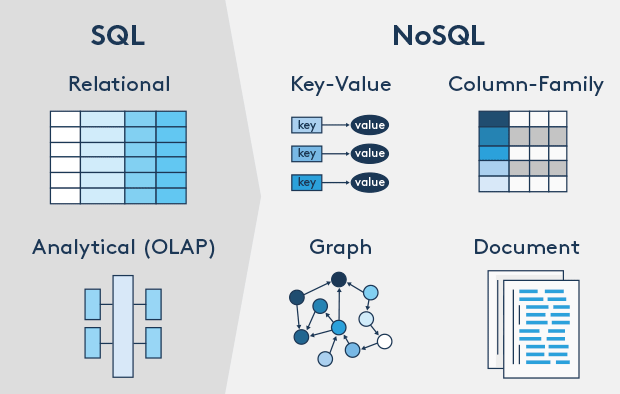
\includegraphics[scale=0.4,clip=true]{sql_vs_nosql}
  \caption{SQL vs NoSQL}
  \label{fig:sql_vs_nosql}
\end{figure}

En realidad, una tabla puede transformarse en documentos, cada uno formado por cada fila de la tabla. Solo es una cuestión de visualización. Lo que pasa es que a menudo en una base de datos no relacional una unidad de datos puede llegar a ser demasiado compleja como para plasmarlo en una tabla.

\subsubsection{Bases de datos SQL}

Las bases de datos SQL son el modelo estándar de toda la vida y también el más utilizado en el mundo tecnológico. SQL es un lenguaje de peticiones estructuradas bastante robusto pero muy poco flexible.

En el ámbito informático se habla mucho de ACID, cuyas siglas vienen de las palabras en inglés: atomicidad, consistencia, aislamiento y durabilidad. Son propiedades que las bases de datos relacionales aportan a los sistemas y les permiten ser más robustos y menos vulnerables ante fallos.

La base de datos relacional más usada y conocida es MySQL junto con Oracle Database, seguida por Microsoft SQL Server, PostgreSQL y SQLite.

Algunas ventajas de las bases de datos SQL son:

\begin{itemize}
  \item Es una tecnología ampliamente conocida y los perfiles que lo conocen son mayoritarios y más económicos.
  \item Mayor soporte y mejores herramientas debido al largo tiempo que llevan en el mercado.
  \item Los datos deben cumplir requisitos de integridad tanto en tipo de datos como en compatibilidad.
  \item La atomicidad de las operaciones en la base de datos. Esto significa que si hay un error durante la petición a cualquier nivel de la operación, se devuelve al punto inicial sin comprometer los datos que fueron utilizados durante el proceso.
\end{itemize}

\subsubsection{Bases de datos NoSQL}

Como su propio nombre indica, las bases de datos NoSQL (Not only SQL) son las que, a diferencia de la relacionales, no tienen un identificador que sirva de relación entre un conjunto de datos y otros. La información se organiza normalmente mediante documentos y es muy útil cuando no tenemos un esquema exacto de lo que se va a almacenar.

Las bases de datos NoSQL son un modelo que se ha puesto muy de moda entre los desarrolladores full-stack porque no requiere un alto conocimiento académico de bases de datos y su curva de aprendizaje y practicidad lo hacen bastante atractivo para proyectos rápidos.

NoSQL se compone generalmente de bases de datos, compuestas a su vez por colecciones que poseen documentos; también hay otras tecnologías NoSQL que poseen columnas y estructuras diferentes.

La indiscutible reina del éxito de las bases de datos NoSQL es MongoDB seguida por Redis, Elasticsearch, CouchDB y Apache Cassandra.

\begin{figure}[htp!]
  \centering
  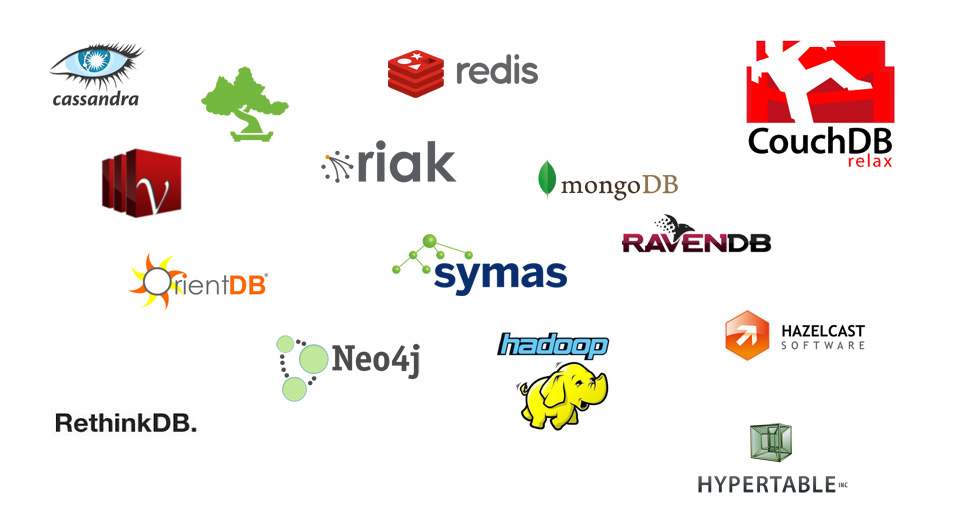
\includegraphics[scale=0.3,clip=true]{nosql_landscape}
  \caption{Panorama de soluciones NoSQL}
  \label{fig:nosql_landscape}
\end{figure}

Algunas ventajas de las bases de datos NoSQL son:

\begin{itemize}
  \item Su naturaleza descentralizada permite una alta escalabilidad. NoSQL es muy utilizada de una amplia forma en aplicaciones con Big Data.
  \item Son mucho más abiertas y flexibles. Permiten adaptarse a necesidades de proyectos mucho más fácilmente que los modelos de Entidad-Relación.
  \item Se pueden hacer cambios de los esquemas sin tener que parar la base de datos.
  \item Escalabilidad horizontal: son capaces de crecer en número de máquinas, en vez de en cantidad de recursos de hardware en una sola máquina.
  \item No necesita altos recursos para ejecutarse. Cualquier servidor con la mínima cantidad de recursos puede correr una base de datos no relacional.
  \item Optimización de consultas en bases de datos para grandes cantidades de datos.
\end{itemize}

\subsection{Serialización de datos}

El universo de servicios y aplicaciones web disponibles hoy en día en Internet es tan inmenso como heterogéneo y muchos de ellos comparten información entre sí. Entonces, ¿cómo logramos que todos estos sistemas, siendo diferentes uno del otro, puedan transmitirse datos? Sencillo, gracias a los formatos de serialización de datos. De no ser por estos estándares creados para representar datos, esta tarea sería un verdadero infierno.

Los sistemas necesitan formatos robustos, que permitan transmitir y compartir información compleja entre sistemas diferentes, con estructuras jerárquicas y atributos variables pero a su vez sean fáciles de leer por un humano. Es aquí donde entran estándares como XML, JSON y YAML.

\begin{figure}[htp!]
  \centering
  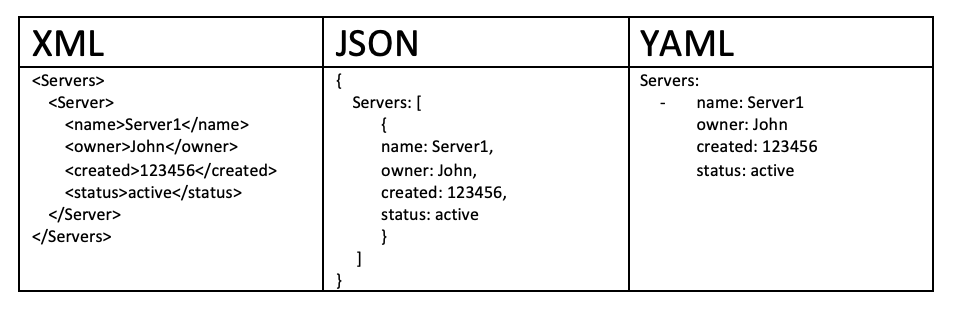
\includegraphics[scale=0.6,clip=true]{xml_json_yaml}
  \caption{XML vs JSON vs YAML}
  \label{fig:xml_json_yaml}
\end{figure}

Los tres formatos de serialización mencionados tienen la misma extensión que su nombre (.xml, .json y .yaml respectivamente). Así que es más fácil de recordar. De hecho, las extensiones de archivo son arbitrarias para los tres estándares de serialización de datos. Es útil para la aplicación y los usuarios saber qué formato de archivos, tipo de contenido y estructura de datos se están utilizando.

Gracias a estos formatos, podemos contar con servicios y aplicaciones que hacen más fácil la vida de desarrolladores y usuarios.

\subsubsection{XML}

XML (del inglés eXtensible Markup Language) es un lenguaje de marcado, al igual que HTML, que define un conjunto de reglas para codificar información de manera que sea legible por un ser humano y por un ordenador.

XML es una evolución que se inició en el lenguaje GML creado por IBM. XML se usa ampliamente para transmitir información entre servicios web y para definir archivos de configuración. Uno de los lenguajes de programación que le da más soporte es Java.

Una de las fortalezas de XML es el soporte a Unicode, lo que permite escribir la información en cualquier idioma del mundo y otra es el amplio soporte que tiene en la actualidad. Sin embargo, ha sido duramente criticado por su verbosidad y complejidad; mapear una estructura básica XML usando tipos de datos de un lenguaje de programación o bases de datos a veces puede ser muy difícil y poco descriptivo.

Los documentos de texto, hojas de cálculo, páginas web y bases de datos son algunos de los campos de aplicación del XML. El metalenguaje aparece como un estándar que estructura el intercambio de información entre las diferentes plataformas.

\subsubsection{JSON}

Es un formato para intercambio de datos, un estándar abierto que utiliza texto plano para codificar información en la forma atributo-valor. Su nombre proviene del inglés JavaScript Object Notation y aunque en sus inicios fue considerado como una parte de JavaScript, siempre ha sido independiente del lenguaje de programación y se encuentra disponible para los lenguajes más populares.

JSON es ampliamente usado para intercambio de información entre servicios web y REST APIs. Es usado especialmente en entornos donde el tamaño del flujo de datos es de vital importancia. Su simplicidad y facilidad de implementación le otorgan un gran desempeño y lo convierten en una de las alternativas ideales al momento de reemplazar XML.

\subsubsection{YAML}

Su nombre proviene del inglés YAML Ain’t Another Markup Language. Es otro formato para el intercambio de información que tiene como objetivo facilitar el mapeo de estructuras de datos más complejas (como las listas) en un documento de texto plano legible por un ser humano. Si bien es un formato joven, sus características le han hecho ganarse un lugar importante en la web, junto con XML y JSON.

YAML es más estricto que los anteriores pero también más simple. Estas características le otorgan elegancia y claridad, haciéndolo ideal para tareas que involucren intervención de un humano.

La simplicidad también le otorga velocidad pero, a diferencia del JSON, no es usado en servicios web sino en archivos de configuración, depuración u otros fines en los que la facilidad de lectura juegan un rol importante.

\subsection{Virtualización}

La mayoría de nosotros cuando escuchamos el concepto de virtualización pensamos inmediatamente en máquinas virtuales, pero es importante entender que este es solo un tipo de virtualización. Entendiendo lo anterior podemos definir los contenedores como otra alternativa de virtualización.

\begin{figure}[htp!]
  \centering
  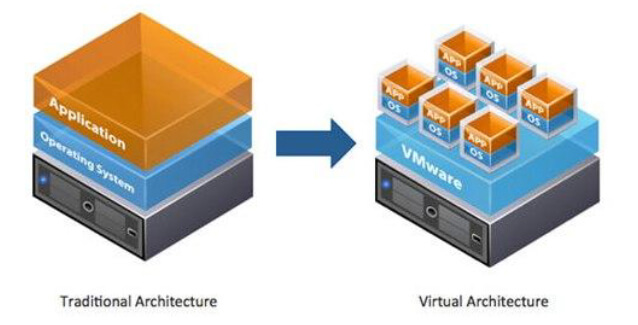
\includegraphics[scale=0.4,clip=true]{vm}
  \caption{Virtualización}
  \label{fig:vm}
\end{figure}

En términos simples los contenedores crean la percepción de un ambiente aislado exclusivo para la aplicación mientras que en la virtualización “tradicional” de máquinas virtuales la aplicación se ejecuta en un sistema operativo virtualizado donde convive con otros aplicativos \cite{docker1}.

\begin{figure}[htp!]
  \centering
  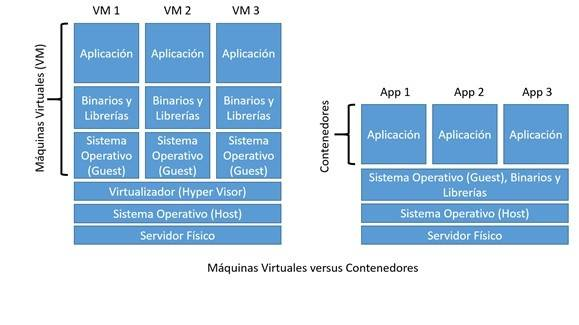
\includegraphics[scale=0.5,clip=true]{vm_container}
  \caption{Máquina virtual vs Contenedor}
  \label{fig:vm_container}
\end{figure}

\subsubsection{Docker}

La idea detrás de Docker es crear contenedores ligeros y portables para las aplicaciones software que puedan ejecutarse en cualquier máquina con Docker instalado, independientemente del sistema operativo que la máquina tenga por debajo, facilitando así también los despliegues \cite{docker4}.

\begin{figure}[htp!]
  \centering
  
\includegraphics[scale=0.1,clip=true]{docker_logo}
  \caption{Logo de Docker}
  \label{fig:docker_logo}
\end{figure}

El propósito de los contenedores es esta independencia: la capacidad de ejecutar varios procesos y aplicaciones por separado para hacer un mejor uso de su infraestructura y, al mismo tiempo, conservar la seguridad que tendría con sistemas separados \cite{docker5}.

Las herramientas del contenedor, como Docker, ofrecen un modelo de implementación basado en imágenes. Esto permite compartir una aplicación, o un conjunto de servicios, con todas sus dependencias en varios entornos.

Digamos que el contenedor de Docker toma los recursos más básicos, que no cambian de un ordenador a otro del sistema operativo de la máquina en la que se ejecuta. Y los aspectos más específicos del sistema que pueden dar más problemas a la hora de llevar el software de un lado a otro, se meten en el interior del contenedor.

Que un contenedor Docker tome los aspectos básicos de funcionamiento del sistema operativo de la máquina en la que se ejecuta lo vuelve más ligero que una máquina virtual.

\begin{figure}[htp!]
  \centering
  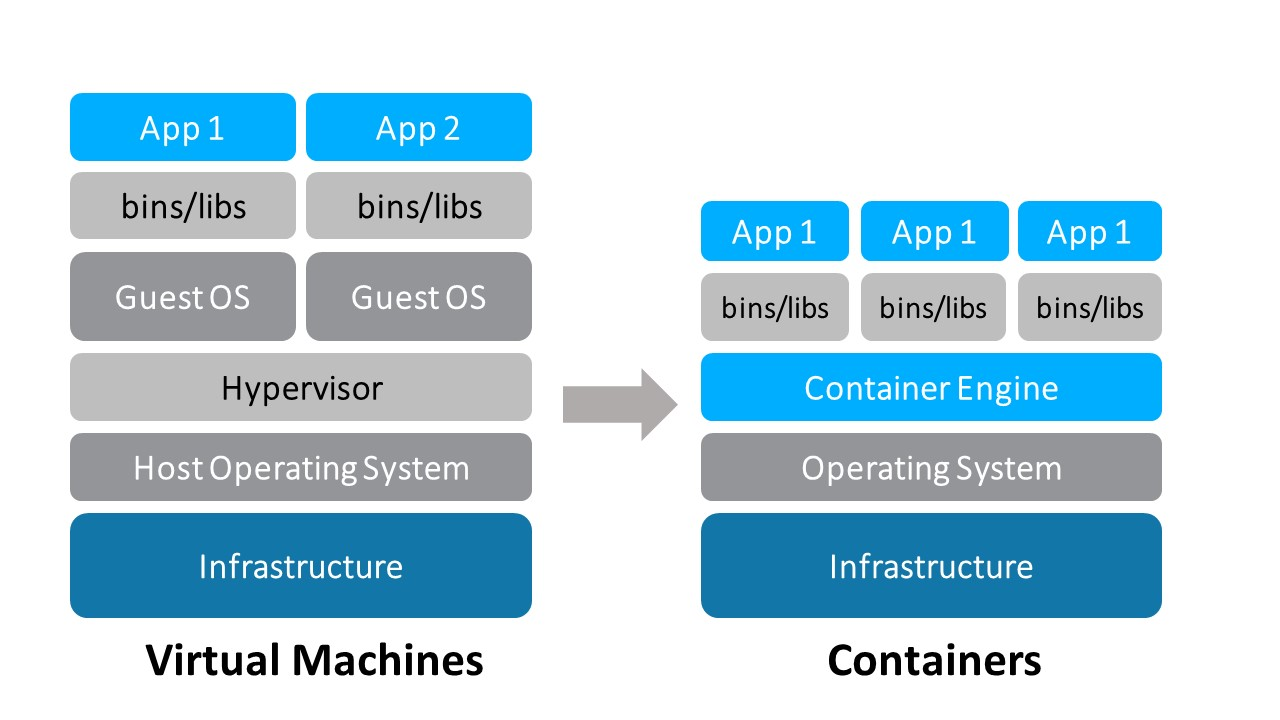
\includegraphics[scale=0.3,clip=true]{vm_vs_docker}
  \caption{Máquina virtual vs Docker}
  \label{fig:vm_vs_docker}
\end{figure}


%
% Diseño
%
\chapter{EVALUACIÓN DE RIESGOS\label{sec:disenho}}

\clearpage

El objetivo principal que busca la ingeniería de software es convertir el desarrollo de software en un proceso formalizado, con resultados predecibles, que permitan obtener un producto final de alta calidad y satisfaga las necesidades y expectativas del cliente.

Por esta razón, una fase importante es la representación simplificada del proceso para el desarrollo y evaluación de la solución software de este proyecto, desde una perspectiva que señala los beneficios y riesgos de las decisiones que tomamos en los diferentes marcos de trabajo.

Como en un modelo de desarrollo de software, este capítulo rescata etapas como la especificación de requisitos, el diseño, la implementación y la evaluación, teniendo en cuenta los objetivos principales de este proyecto.

\begin{figure}[htp!]
  \centering
  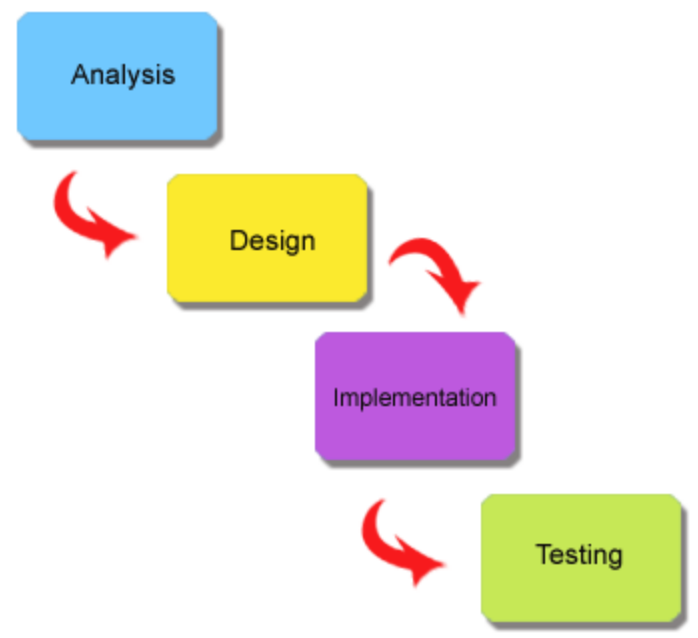
\includegraphics[scale=0.2,clip=true]{waterfall_model}
  \caption{Modelo de desarrollo de software}
  \label{fig:waterfall_model}
\end{figure}

\section{Identificación de los requisitos}

Los requisitos no funcionales tienden a ser aquellos que reflejan la calidad del producto. Especifican los criterios que pueden usarse para juzgar el funcionamiento de un sistema como por ejemplo la disponibilidad, accesibilidad, usabilidad, mantenibilidad, seguridad o rendimiento.

\subsection{Mensajería instantánea}

En la actualidad la mensajería instantánea cada vez tiene una mayor presencia en las empresas. Esta situación hace necesaria la adopción de una serie de requisitos a la hora de autorizar el uso de estos servicios. A continuación se detallan algunos de éstos requisitos:

\begin{itemize}
  \item Confidencialidad de la comunicación. Los mensajes transmitidos a través del servicio de mensajería instantánea sólo pueden ser leídos por el receptor, estableciendo las medidas de seguridad que sean necesarias para evitar que terceros puedan acceder a su contenido.
  \item Integridad del mensaje. Los mensajes no deben poder ser alterados.
  \item Identificación. Los mensajes deben contener la información de su emisor y la persona a la que va dirigido, evitando que el mensaje sea entregado a un destinatario equivocado.
  \item El emisor no debe poder modificar ni eliminar un mensaje ya enviado.
\end{itemize}

\subsection{Centro 112 de Madrid}

A día de hoy, el Centro 112 de Madrid, está consagrado como una gran central de gestión de emergencias que ofrece confianza y seguridad a los ciudadanos. Por lo que nos puede servir como punta de partida en la identificación de los requisitos no funcionales.

Los aspectos más destacados del Centro 112 de Madrid son:

\begin{itemize}
  \item Funciona 24 horas al día y 365 días al año.
  \item Cuenta con 241 profesionales, a los que se suman otros 200 de otros cuerpos y servicios de emergencias que también tienen presencia en el mismo centro de operaciones.
  \item Atiende más de 4,5 millones de llamadas al año, según las últimas publicaciones, y el tiempo medio de respuesta, desde que se establece la llamada al 112 y el operador responde, es de tan solo 8 segundos. Y, que en 70 segundos, el operador ha enviado la emergencia al servicio correspondiente.
  \item La sala de equipos está equipada con herramientas de integración de la telefonía en los puestos de trabajo (PCs), para facilitar el trabajo al operador de emergencias mediante el uso exclusivo de pantalla, teclado y ratón.
  \item Tiene incorporado en su Sistema Integrado de Gestión de Emergencias (SIGE112) la app My112, permitiendo la localización del llamante mediante las coordenadas desde donde se está realizando la llamada.
  \item Su modelo 112 está diseñado con criterios de escalabilidad.
\end{itemize}

Teniendo en cuenta esta información relevante, podemos definir los siguientes requisitos no funcionales que la solución software debe cumplir en todo momento:

\begin{itemize}
  \item Funcionamiento: durante 24 horas seguidas.
  \item Participantes en la comunicación: entre dos o más personas.
  \item Tiempo medio de respuesta: 8 segundos.
  \item Duración media de la comunicación: 70 segundos.
  \item Comunicaciones simultáneas: alrededor de 250.
\end{itemize}

\section{Diseño del protocolo de mensajería instantánea}

Desde hace tiempo se sabe que XML es un formato obsoleto y fallido para la serialización de datos intercambiables. Aunque, proporciona todas las características que XMPP necesita, XML no deja de tener su parte de detractores. De hecho, hace algunos años, esto llevó al intento de proporcionar una codificación binaria para XMPP llamada Binary XMPP.

Desafortunadamente, la codificación binaria carecía de las principales ventajas de XML en su legibilidad humana, por lo que la búsqueda de mejores codificaciones nos lleva a JSON.

Por otro lado, si en nuestro proyecto no fuese crítico la comunicación inmediata, sería una buena idea respaldarse en la simplicidad del long pooling. Algunos desarrolladores prefieren usar long pooling porque las tecnologías modernas como son los WebSockets son más complejas y difíciles de configurar. Cuando la simplicidad no es tan importante como el rendimiento, hay que considerar el uso de WebSockets.

\subsection{Mensajería instantánea grupal}

Hoy en día, hay aplicaciones para casi cualquier cosa, incluidas aplicaciones como WhatsApp que te permiten conectarte con dos o más personas al mismo tiempo. Una de las características destacadas de estas aplicaciones de mensajería instantánea es que permiten que grupos grandes hablen y conversen al mismo tiempo. Conocidas como mensajería instantánea grupal, estas aplicaciones las ofrecen de forma predeterminada sin costo.

Dada la naturaleza competitiva de la industria, hay varias aplicaciones que realizan una función similar. Con la multitud de aplicaciones que existen, puede ser bastante difícil elegir una aplicación como base para nuestro desarrollo. Teniendo esto en cuenta, es esencial que nuestra aplicación permita como mínimo el envío de mensajes de texto en un grupo.

\subsection{WebSocket}

Como se ha visto, WebSocket permite establecer comunicaciones bidireccionales en tiempo real en la Web, posibilidad que antes solo existía de forma simulada y bastante costosa mediante técnicas como long polling.

Optar por WebSocket permite reducir la saturación de cabeceras que ocurriría si se utilizase HTTP en su lugar, especialmente para aplicaciones web que requieren un gran volumen de comunicaciones. Además, evita que cada aplicación web utilice una solución de integración diferente, con los problemas de compatibilidad que ello conlleva.

También, se ha visto que su funcionamiento es extremadamente sencillo: se establece una conexión, se envían/reciben mensajes y se cierra la conexión. Al funcionar bajo los mismos puertos que HTTP evita problemas relacionados con cortafuegos, facilitando así el funcionamiento de productos basados en SOA, entre otros.

Por otra parte, es necesario gestionar y mantener un gran número de conexiones que han de permanecer abiertas mientras ambas partes sigan interactuando. Esto puede llegar a ser un problema en determinados casos, teniendo en cuenta que el número máximo de conexiones simultáneas que admite un puerto TCP es de 64.000 y que, además, mantener las conexiones abiertas requiere memoria del servidor.

Por tanto, WebSocket es la mejor solución para aplicaciones web que necesitan actualizaciones constantes en tiempo real como chats, juegos multijugador en línea o retransmisiones interactivas en directo.

\subsection{JSON}

Originalmente, el lenguaje XML era increíblemente flexible y fácil de escribir, pero su inconveniente era que era detallado, difícil de leer para los humanos, muy difícil de leer para los servidores, y tenía mucha sintaxis que no era del todo necesaria para comunicar información.

Hoy en día, XML está muerto para la serialización de datos en la web. A menos que esté escrito en HTML o SVG, ambos hermanos en XML, probablemente no verás XML en otros lugares. Algunos sistemas obsoletos todavía lo usan hoy, pero usarlo para pasar datos tiende a ser excesivo para la web.

La transferencia de datos es mucho más fácil cuando los datos se almacenan en una estructura que está familiarizada a los lenguajes orientados a objetos por lo que es muy sencillo importar datos desde un fichero JSON a Perl, Ruby, JavaScript, Python, y otros muchos lenguajes. En XML, tendríamos que transformar los datos antes de importarlos. Por esta razón, JSON es un formato de fichero superior para las Web APIs.

JSON se usa en todas partes hoy en día. El formato es fácil de escribir tanto por humanos como por máquinas, y se convirtió en el estándar de facto para transferir datos de un sistema a otro. Casi todos los lenguajes de programación tienen una funcionalidad incorporada para leerlos y escribirlos.

Otra de las grandes ventajas que presenta JSON es el rendimiento, ya que los JSON son considerablemente más livianos en peso y mucho más rápido en su procesamiento. Pero como ya vimos, el rendimiento tiene un coste y es la robustez del mensaje como tal.

Un objeto JSON es un objeto válido en JavaScript por lo que es el formato perfecto para este lenguaje. La mayoría de los navegadores web modernos incluyen funciones nativas para codificar y decodificar JSON, lo que le da un punto de ventaja en lo que se refiere a desempeño y disminuyen los riesgos de seguridad.

\section{Desarrollo de la aplicación web en tiempo real}

Una aplicación web en tiempo real requiere un esfuerzo de ingeniería muy grande. En un modelo tradicional son los clientes los que preguntan al servidor, lo que requiere poco trabajo por parte de éste. Las peticiones llegan y el servidor responde. Fácil y sencillo. El servidor no procesa más datos de los necesarios para dar la información que piden los clientes.

Cuando pasamos al modelo del tiempo real, las cosas cambian. Ahora el servidor tiene que preocuparse de dar la información a los clientes cuando ésta se genera. Para ello necesita un registro de clientes que tienen que recibir esa información, así que no sólo tiene que procesar los datos relativos a la información que va a dar sino que además tiene que preocuparse de decidir con quién conectar y cuándo hacerlo. No sólo eso, también tiene que gestionar las conexiones y desconexiones del sistema. Es decir, un método mucho más complejo que el tradicional.

Con toda esa complejidad del tiempo real, alguna ventaja tenía que darnos. La primera es para los servidores. En una aplicación web tradicional, por ejemplo, si de repente los 200.000 clientes de un servicio deciden hacer una petición todos a la vez, el servidor puede bloquearse por saturación. Sin embargo, si son los servidores los que gestionan las conexiones estas situaciones no pueden ocurrir: el servidor distribuye de forma normal las conexiones de forma que no haya problemas de saturación, y evitando los ataques DDoS involuntarios.

La siguiente ventaja es bastante obvia: la instantaneidad de la información. Cuando son las aplicaciones las que tienen que preguntar al servidor, normalmente lo hacen a intervalos usando pooling. Si vamos encadenando varias aplicaciones, los intervalos se acumulan y podemos tener retardos bastante grandes. Con una aplicación web en tiempo real, estos intervalos desaparecen y la información llega con un retraso mínimo.

Otra ventaja es que genera menos tráfico de red. Por ejemplo, si un cliente de correo comprueba cada cinco minutos si tiene mensajes nuevos, cada cinco minutos va a estar generando tráfico haya o no haya mensajes nuevos. Es decir, que estará creando bastante tráfico inútil. Sin embargo, si es el servidor el que avisa al cliente, sólo se produce tráfico cuando hay correo nuevo. De este modo, el tráfico generado es siempre tráfico útil.

\subsection{REST}

REST es una tecnología que transporta datos por medio del protocolo HTTP. Es tan flexible que permite transmitir prácticamente cualquier tipo de datos, ya que el tipo de datos está definido por la cabecera Content-Type, lo que nos permite mandar formatos como XML o JSON, binarios (imágenes, documentos), texto plano, entre otros más.

\begin{figure}[htp!]
  \centering
  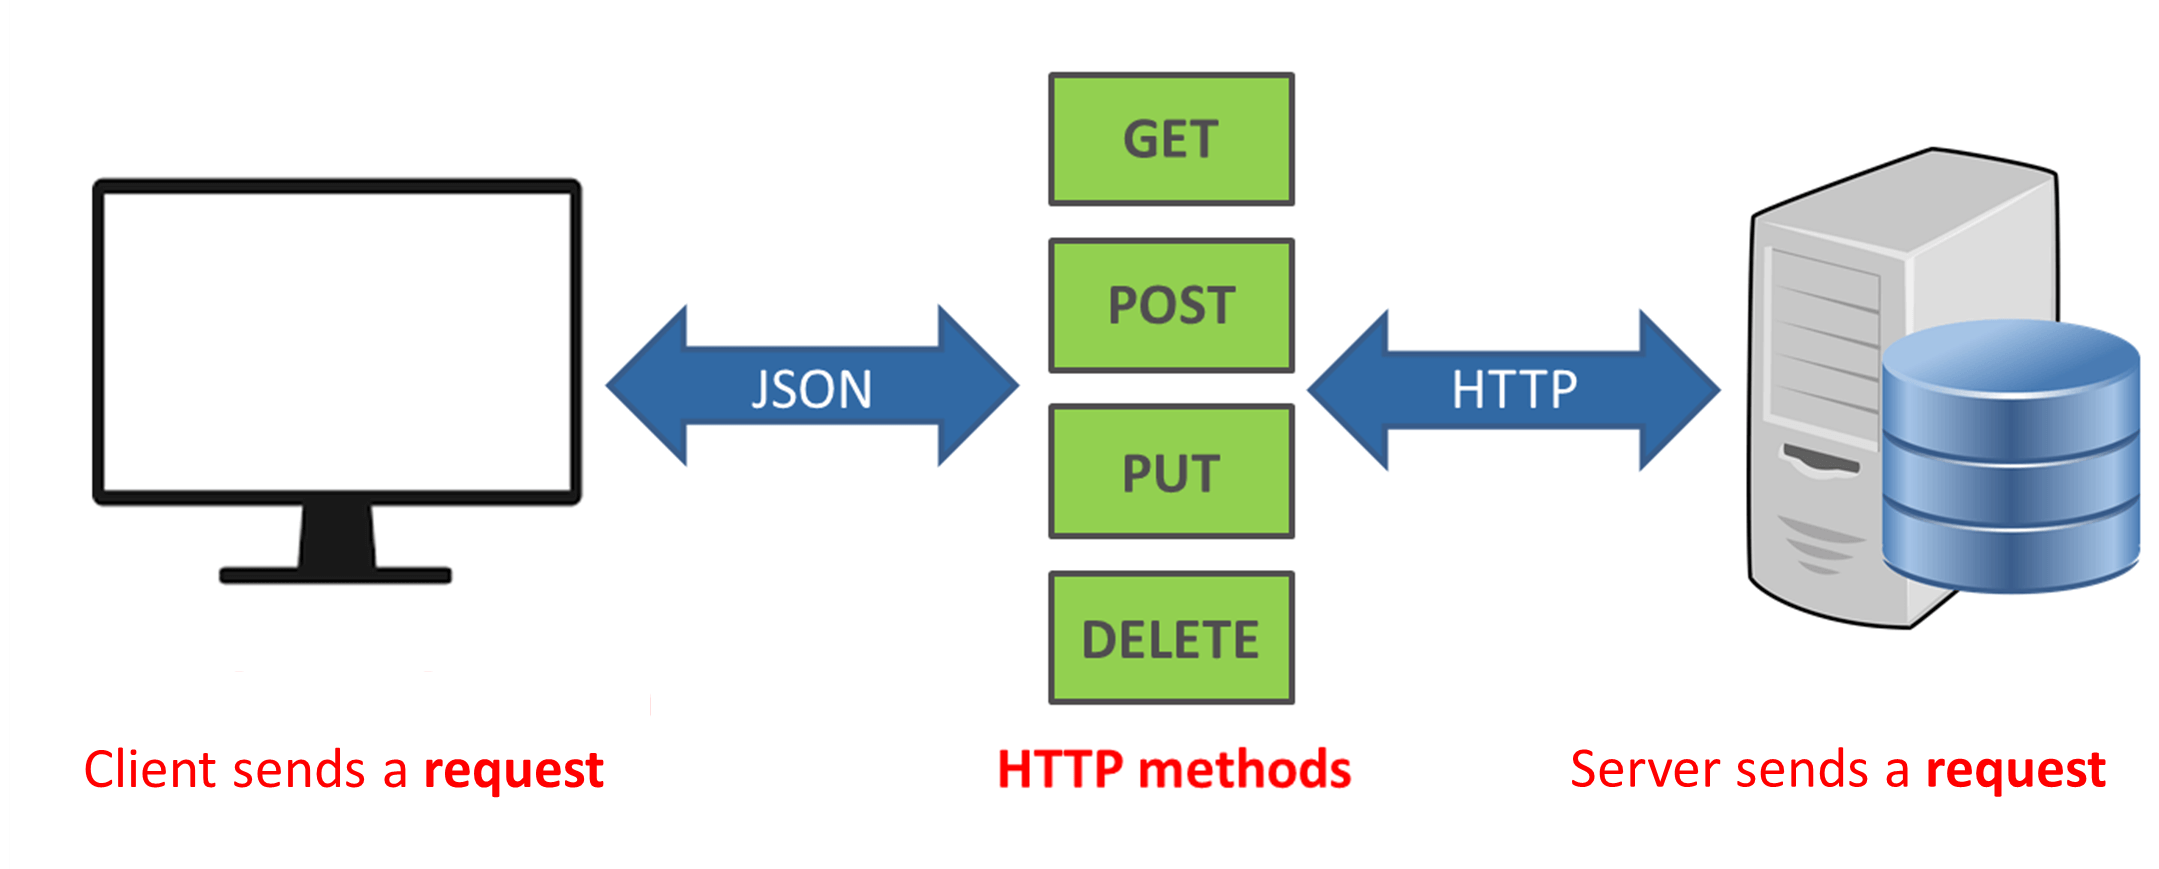
\includegraphics[scale=0.1,clip=true]{rest}
  \caption{Arquitectura de REST}
  \label{fig:rest}
\end{figure}

REST se caracteriza por no tener estado. Es decir, el servidor no es capaz de recordar el estado de la anterior solicitud REST que pudo, o no, hacer un cliente. Por ello, el cliente tiene que enviar en cada solicitud todo el estado de su sesión.

REST viene para simplificar las cosas. Hoy REST y JSON se han convertido en la opción más sencilla y por tanto más recomendable para implementar una aplicación web.

\subsection{Node.js}

Gracias a que Node.js permite trabajar tanto desde el servidor como desde el cliente, es posible generar una transferencia de información mucho más rápida e inmediata. El resultado de todo esto es una reducción considerable en los periodos de trabajo.

Además al ser un lenguaje popular y empleado por profesionales de todo el mundo resulta fácil encontrar información y recursos en Internet. Está diseñado para incentivar el intercambio entre usuarios y programadores.

Es quizá la opción más competitiva para diseñar aplicaciones que gestionan grandes cantidades de información generadas por una comunidad elevada de usuarios.

Debido a sus altas prestaciones para gestionar y procesar grandes volúmenes simultáneos de información, Node.js es una opción estrella para el desarrollo de aplicaciones como chats online.

\subsubsection{Beneficios de utilizar Node.js}

Asumiendo que lo que interesa son las ventajas desde el punto de vista del desarrollo web, a continuación se definen las más significativas:

\begin{itemize}
  \item Escalabilidad de manera sencilla. Node.js se diseñó con una arquitectura dirigida por eventos y con E/S asíncrona desde el minuto 0. Eso hace que sea muy escalable de forma sencilla y directa.
  \item Rendimiento. Gracias al motor V8 el uso de Javascript en Node.js supera a soluciones basadas en otros lenguajes “interpretados”.
  \item Javascript. Node.js está basado en Javascript, que es un lenguaje que está de moda, en parte gracias al propio Node.js. Y además es el lenguaje de la web. El único soportado por todos los navegadores. Ahora que las aplicaciones web se han hecho muy interactivas y que es ingente la cantidad de código en Javascript que corre en los navegadores, es muy cómodo poder desarrollar con el mismo lenguaje en el servidor.
  \item Popularidad. Como he mencionado todo esto ha llevado a que Node.js y Javascript gocen de gran popularidad. Cada vez hay más interés y más desarrolladores. Y eso hace que la comunidad sea enorme, lo que es muy interesante en caso de necesitar ayuda.
\end{itemize}

\subsubsection{Event Loop de Node.js}

Si una empresa desea que su aplicación soporte más usuarios, necesitará agregar más y más servidores. Por todas estas razones, el cuello de botella en toda arquitectura de aplicaciones web es el número máximo de conexiones concurrentes que podía manejar un servidor.

Node.js resuelve este problema cambiando la forma en que se realiza una conexión con el servidor. En lugar de generar un nuevo hilo del sistema operativo para cada conexión (y de asignarle la memoria acompañante), cada conexión dispara una ejecución de evento dentro del proceso del motor V8 de Node.js.

Node.js emplea un único hilo y un event loop asíncrono. Las nuevas peticiones son tratadas como eventos en este bucle. Este es el motivo por el que las características asíncronas y los eventos de JavaScript encajan tan bien en la filosofía de Node.js.

\begin{figure}[htp!]
  \centering
  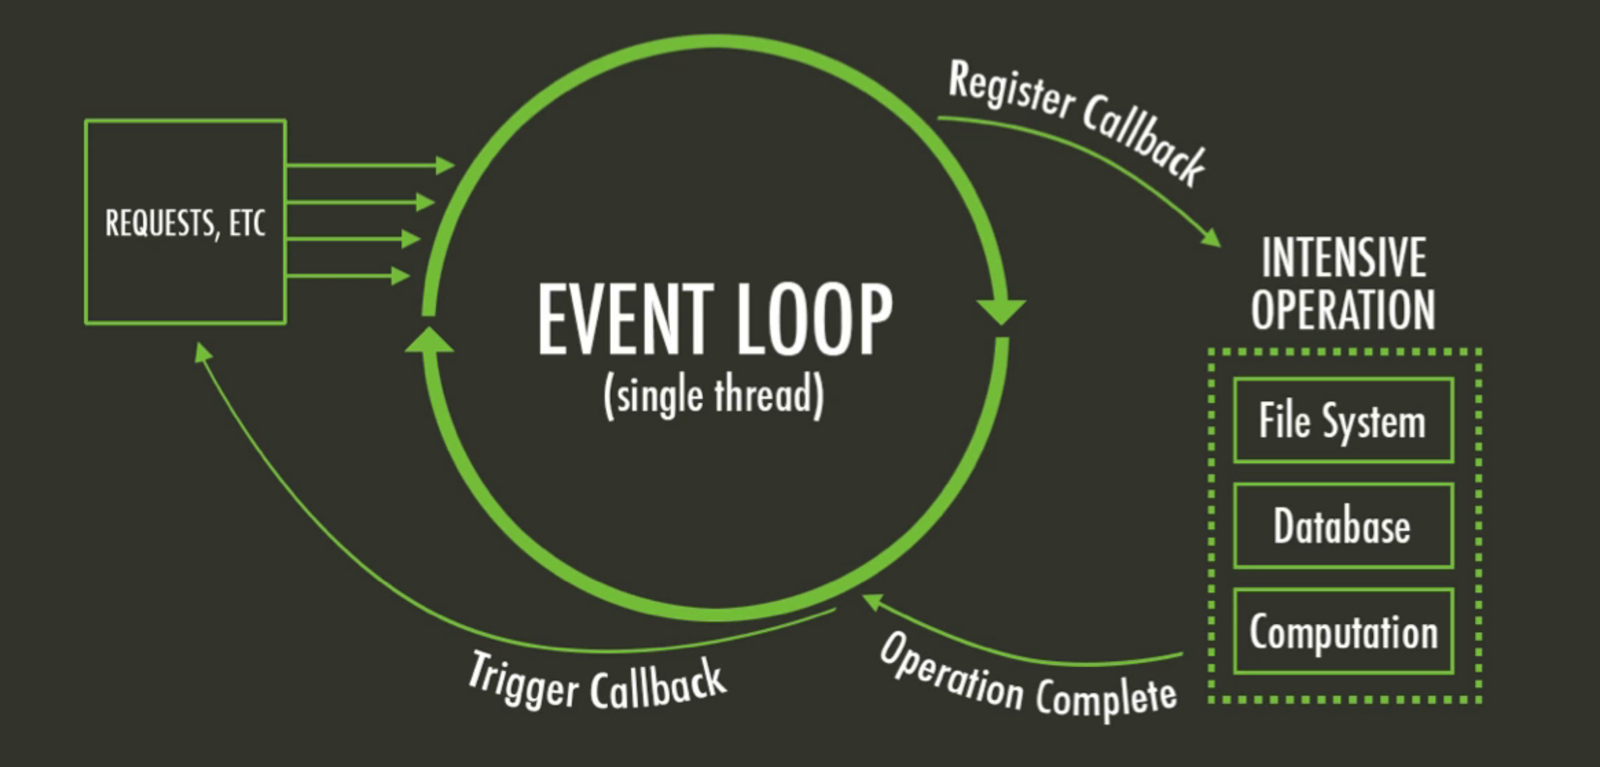
\includegraphics[scale=0.2,clip=true]{nodejs_eventloop}
  \caption{Event Loop de V8}
  \label{fig:nodejs_eventloop}
\end{figure}

Esto permite que Node.js sea capaz de gestionar múltiples conexiones y peticiones de forma muy eficiente, lo que lo hace apropiado para desarrollo y aplicaciones con un gran número de conexiones simultáneas.

\subsubsection{NPM}

En un proyecto Node.js, el código se organiza por módulos o paquetes, así que al momento de trabajar con él va a ser necesario agregar más módulos, es aquí donde entra la herramienta NPM.

\begin{figure}[htp!]
  \centering
  
\includegraphics[scale=0.05,clip=true]{npm_logo}
  \caption{Logo de NPM}
  \label{fig:npm_logo}
\end{figure}

Node Package Manager, o simplemente npm, es un gestor de paquetes, el cual hará más fácil nuestras vidas al momento de trabajar con Node.js, ya que gracias a él podremos tener cualquier librería disponible con solo una línea de código. NPM nos ayudará a administrar nuestros módulos, distribuir paquetes y agregar dependencias de una manera sencilla.

\subsubsection{Express.js}

Muchos desarrolladores de software han optado por utilizar JavaScript para construir aplicaciones web. Esto ha provocado un crecimiento exponencial de los frameworks web para Node.js con el objetivo de facilitar la creación rápida de prototipos y la construcción de aplicaciones web impresionantes, especialmente en el lado del servidor.

Los frameworks para Node.js se utilizan principalmente debido a su productividad, escalabilidad y velocidad, lo que los convierte en una de las primeras opciones para crear aplicaciones web para empresas.

Al usar un framework, puedes trabajar con un conjunto de herramientas, directrices y prácticas recomendadas que lo ayudan a ahorrar tiempo. También puede ayudar a consolidar los estándares de código en un equipo de desarrolladores.

Express.js es un framework web rápido, flexible y minimalista para Node.js. Es simplemente una tecnología basada en Node.js que se comporta como un middleware para ayudar a administrar nuestros servicios y rutas.

\begin{figure}[htp!]
  \centering
  
\includegraphics[scale=0.2,clip=true]{express_logo}
  \caption{Logo de Express.js}
  \label{fig:express_logo}
\end{figure}

Express.js ha demostrado, con el tiempo, que su popularidad vale la pena con sus métodos y funciones fáciles de usar. Probablemente sea el framework web para Node.js más popular disponible para la comunidad de JavaScript en GitHub con más de 41,000 estrellas.

Algunas de las numerosas ventajas de Express.js incluyen:

\begin{itemize}
  \item Casi el estándar para el middleware web de Node.js.
  \item Totalmente personalizable.
  \item Curva de aprendizaje baja.
\end{itemize}

\subsection{MongoDB}

Es muy común entre los desarrolladores de aplicaciones web encontrarse en la situación de tener que elegir si se va a usar una base de datos SQL o NoSQL. La mayoría no se lo piensa demasiado y opta por la opción que mejor conocen y con la que más cómodos trabajan. Tampoco es una decisión catastrófica; en realidad, ya sea una base de datos SQL o NoSQL, se puede construir cualquier cosa.

Es importante saber en qué se diferencian y cuál deberíamos usar en cada caso, ya que un buen diseño de base de datos con la tecnología apropiada indudablemente aporta calidad al proyecto. Dependiendo de la naturaleza de la aplicación, interesa que la base de datos tenga unas características u otras.

La diferencia fundamental entre ambos tipos de base de datos radica en que las bases de datos NoSQL no hacen uso de un modelo relacional. Si tu proyecto necesita una escalabilidad importante, donde los recursos son escasos y no necesita respetar la integridad de los datos, entonces sí: NoSQL es la mejor opción.

A la hora de hacer una aplicación web, existen varias soluciones para cada uno de los grandes componentes que forman una aplicación completa. Si el servidor web está en Node.js, MongoDB es la base de datos NoSQL que tiene más éxito entre este tipo de aplicaciones.

\begin{figure}[htp!]
  \centering
  
\includegraphics[scale=0.1,clip=true]{mongodb_logo}
  \caption{Logo de MongoDB}
  \label{fig:mongodb_logo}
\end{figure}

\subsubsection{Beneficios de MongoDB}

Los siguientes son algunos de los beneficios y fortalezas de MongoDB:

\begin{itemize}
  \item Esquema dinámico. como se mencionó, esto le brinda flexibilidad para el esquema de los datos sin modificar ninguno de los datos ya existentes.
  \item Escabilidad. MongoDB es escalable horizontalmente, lo que ayuda a reducir la carga de trabajo y la escala de tu negocio con facilidad.
  \item Capacidad de administración. la base de datos no requiere un administrador de base de datos. Ya que es bastante fácil de usar de esta manera, puede ser utilizado tanto por desarrolladores como por administradores.
  \item Velocidad. Es de alto rendimiento para consultas simples.
  \item Flexibilidad. puede agregar nuevas columnas o campos en MongoDB sin afectar las filas existentes o el rendimiento de la aplicación.
\end{itemize}

\subsection{Docker}

Aunque, por su naturaleza, se asemejan a las clásicas máquinas virtuales, estamos hablando de algo más avanzado porque nos ofrecen una mayor eficiencia y sencillez.

Para empezar, los contenedores de Docker comparten recursos con el sistema operativo sobre el que se ejecutan. De esta manera podemos arrancar o parar el contenedor rápidamente, mientras que las máquinas virtuales se aíslan del sistema operativo sobre el que trabajan y se comunican a través del hypervisor \cite{docker2}.

La portabilidad de los contenedores hace que los problemas causados por cambiar el entorno donde está corriendo la aplicación se reduzcan a la mínima expresión.

En cuanto al rendimiento, existen diferencias respecto a una virtualización de máquina completa. Los tiempos de arranque son menores. Además, el nivel de aislamiento es menor y ciertas partes de la memoria del contenedor están duplicadas, lo que permite ejecutar múltiples instancias del mismo contenedor sin que ello suponga una gran merma de la memoria.

\subsubsection{Ventajas de los contenedores de Docker}

Las ventajas de los contenedores Docker son:

\begin{itemize}
  \item Modularidad. El enfoque Docker para la creación de contenedores se centra en la capacidad de tomar una parte de una aplicación, para actualizarla o repararla, sin necesidad de tomar la aplicación completa.
  \item Control de versiones de imágenes y capas. Cada archivo de imagen de Docker se compone de una serie de capas. Estas capas se combinan en una sola imagen. Una capa se crea cuando la imagen cambia. Docker reutiliza estas capas para construir nuevos contenedores, lo cual hace mucho más rápido el proceso de construcción.
  \item Restauración. Probablemente la mejor parte de la creación de capas es la capacidad de restaurar. Si no te gusta la iteración actual de una imagen, restaura la versión anterior.
  \item Implementación rápida. Solía demorar días desarrollar un nuevo hardware, ejecutarlo, proveerlo y facilitarlo. Y el nivel de esfuerzo y sobrecarga era extenuante. Los contenedores basados en Docker pueden reducir el tiempo de implementación a segundos.
\end{itemize}

\section{Diseño del entorno de pruebas}

Una vez que tengamos probada y desplegada nuestra aplicación, se debe probar de forma automática las capacidades y debilidades del software y de la plataforma sobre la que está corriendo (infraestructura y dependencias), llevándola al límite, para comprobar su disponibilidad, estabilidad y resiliencia.

\subsection{Pruebas no funcionales}

Las pruebas no funcionales se refieren a aspectos del software que pueden no estar relacionados con una función específica o acción del usuario, como la escalabilidad o el comportamiento bajo ciertas restricciones o la seguridad. Estas pruebas determinan el punto de ruptura, el punto en el que los extremos de escalabilidad o rendimiento llevan a una ejecución inestable.

Podemos clasificar las pruebas no funcionales según el tipo de requisito no funcional que abarcan:

\subsubsection{Pruebas de seguridad}

Las pruebas de seguridad validan los servicios de seguridad de una aplicación e identifican posibles fallos y debilidades. Las pruebas de seguridad son esenciales para el software que procesa datos confidenciales para evitar la intrusión en el sistema por parte de hackers informáticos.

Muchos proyectos utilizan un enfoque de caja negra para las pruebas de seguridad, lo que permite a los expertos, sin conocimiento del software, probar la aplicación en busca de agujeros, fallos, exploits y debilidades.

\subsubsection{Pruebas de usabilidad}

Las pruebas de usabilidad son para verificar si la interfaz de usuario es fácil de usar y entender. Se refiere principalmente a la interacción con la aplicación. Este no es un tipo de prueba que se pueda automatizar; se necesitan usuarios reales, que sean monitoreados por diseñadores de interfaces de usuario expertos.

\subsubsection{Pruebas de rendimiento}

Las pruebas de rendimiento verifican la capacidad de respuesta, el rendimiento, la confiabilidad y/o la escalabilidad del sistema cuando está bajo una carga de trabajo significativa.

Por su naturaleza, las pruebas de rendimiento pueden ser bastante costosas de implementar y ejecutar, pero pueden ayudarte a entender si los nuevos cambios van a degradar o mejorar el rendimiento del sistema.

En aplicaciones web, las pruebas de rendimiento a menudo están estrechamente relacionadas con las pruebas de estrés, la medición del retraso y la capacidad de respuesta bajo una carga pesada. Por ejemplo, se pueden observar los tiempos de respuesta cuando se ejecuta una gran cantidad de peticiones de usuario, o ver cómo se comporta el sistema con una cantidad significativa de datos.

\subsection{Diseño de pruebas de rendimiento}

Las pruebas de rendimiento generalmente se ejecutan para determinar cómo se desempeña un sistema o subsistema en términos de capacidad de respuesta y estabilidad bajo una carga de trabajo en particular. Pero, también puede servir para investigar, medir, validar o verificar otros atributos de calidad del sistema, como la escalabilidad, la confiabilidad y el uso de recursos.

\subsubsection{Pruebas de carga}

Las pruebas de carga se encarga principalmente de comprobar que el sistema puede continuar operando bajo una carga de trabajo específica, ya sea en grandes cantidades de datos o en una gran cantidad de peticiones. Esta carga puede ser el número esperado de usuarios concurrentes, que utilizando la aplicación realizan un número específico de transacciones durante el tiempo que dura la carga.

Una prueba de carga puede mostrar los tiempos de respuesta de todas las transacciones importantes de la aplicación. Esto generalmente se conoce como escalabilidad de software.

Si también se monitorizan otros aspectos como la base de datos, el servidor de aplicaciones, etcétera, entonces esta prueba puede mostrar el cuello de botella de la aplicación.

\subsubsection{Pruebas de estrés}

La prueba de estrés empuja los límites funcionales de un sistema. Se realiza sometiendo el sistema a condiciones extremas, como volúmenes de datos máximos o una gran cantidad de usuarios simultáneos. Se utiliza normalmente para romper la aplicación.

Se va doblando el número de usuarios que se agregan a la aplicación y se ejecuta una prueba de carga hasta que se rompe. Esto ayuda a los administradores para determinar si la aplicación rendirá lo suficiente en caso de que la carga real supere a la carga esperada.

También se utilizan para, llevado el sistema al colapso o degradación, comprobar su funcionamiento continuado por encima de su límite y, una vez liberado de la carga, evaluar su capacidad de resiliencia volviendo a su estado óptimo de funcionamiento.

\subsubsection{Pruebas de estabilidad}

Las pruebas de estabilidad o soak testing comprueban si el software puede funcionar continuamente en un período aceptable o superior; es decir, si la aplicación puede aguantar una carga esperada continuada. Generalmente esta prueba se realiza para determinar si hay alguna pérdida de memoria (memory leak) en la aplicación.

Las pruebas de estabilidad son una gran prueba, que a menudo se pasa por alto, y que muestra muchos aspectos críticos sobre una aplicación bajo carga de trabajo constante, cosas que ninguna otra prueba puede y es crítica para determinar si la aplicación es apta para la producción.

Hay que tener en cuenta los requisitos de la aplicación, la organización y la producción para determinar el largo periodo de tiempo que la prueba de estabilidad estará ejecutándose.

En una organización en la que los sistemas de producción se apagan y reinician todas las noches, la prueba de estabilidad no debe durar más de 24 horas. En cambio, si la aplicación se reinicia semanalmente como parte de un ciclo de mantenimiento, entonces la prueba de estabilidad debe durar al menos 7 días.

\subsection{Herramienta para pruebas de rendimiento}

Existen numerosas herramientas, tanto open source como privadas, para realizar las pruebas de rendimiento: NeoLoad, LoadRunner, LoadUI, WebLOAD, Artillery, etcétera. Una de las más populares es Apache JMeter.

Apache JMeter es una herramienta para llevar a cabo simulaciones sobre cualquier recurso de software. Es una herramienta creada por Apache y está completamente escrita en Java.

\begin{figure}[htp!]
  \centering
  
\includegraphics[scale=0.3,clip=true]{jmeter_logo}
  \caption{Logo de Apache JMeter}
  \label{fig:jmeter_logo}
\end{figure}

Apache Jmeter se suele usar para hacer pruebas de carga aunque también soporta aserciones para asegurar que los datos recibidos son correctos y muchas posibilidades a la hora de generar reportes.

\subsubsection{Java}

TODO


%
% Desarrollo
%
\chapter{DESARROLLO\label{sec:desarrollo}}

TODO: Desarrollo del proyecto

\subsection{Prueba de carga}

TODO: Alcance del trabajo/proyecto

\subsubsection{Protocolo WebSocket}

TODO: Alcance del trabajo/proyecto

\section{Motivaciones del proyecto}

TODO: Estado del arte

\subsection{Motivaciones del proyecto}

TODO: Alcance del trabajo/proyecto

\subsubsection{Motivaciones del proyecto}

TODO: Alcance del trabajo/proyecto

\paragraph{Motivaciones del proyecto}

TODO: Alcance del trabajo/proyecto


%
% Resultados
%
\chapter{RESULTADOS\label{sec:resultados}}

\clearpage

Este capítulo analiza los resultados de las pruebas no funcionales centradas en el rendimiento de la aplicación web de mensajería instantánea desarrollada en el capítulo anterior. Para, posteriormente, justificar si la solución web propuesta en este documento cumple con los requisitos mínimos de integración en las aplicaciones de emergencias para teléfonos móviles.

Seguimos con la metodología de pruebas de rendimiento según Microsoft Developer Network. Ya hemos ejecutado y monitorizado las pruebas. Hemos recogido los resultados y vamos con el último paso.

\section{Analizar los resultados y realizar un informe}

En la última fase, se consolida y comparte los resultados de la prueba. Analizamos los datos, tanto individualmente como con un equipo multidisciplinario. Volvemos a priorizar el resto de las pruebas y a ejecutarlas en caso de que sea necesario.

Cuando todas las métricas estén dentro de los límites aceptados, ninguno de los umbrales establecidos hayan sido rebasados y toda la información deseada se ha reunido, las pruebas han acabado para el escenario definido por la configuración \cite{jmeter6}.

Ahora que tenemos los resultados, vamos a destacar tres casos.

\subsection{Prueba de 300 salas, 10 usuarios por sala y 1 mensaje cada 2,5 segundos}

El primer caso es el caso más extremo que podría darse en un centro 112, ya que tendríamos todos los operadores (300) usando el servicio de IM, al mismo tiempo que también personal de soporte (digamos que 10 usuarios por sala) y enviando mensajes con una frecuencia real (1 mensaje cada 2,5 segundos).

\begin{figure}[htp!]
  \centering
  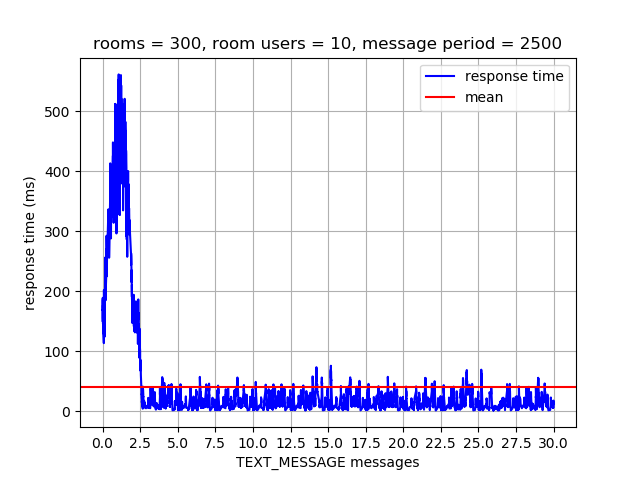
\includegraphics[scale=0.6,clip=true]{chat_r300_u10_m2500}
  \caption{Prueba de 300 rooms, 10 room users y 2500 msg period}
  \label{fig:chat_r300_u10_m2500}
\end{figure}

Como podemos observar en la gráfica, al principio el tiempo de respuesta es peor ya que el sistema se prepara y luego reutiliza recursos por lo que el resto de mensajes ya tienen un tiempo más similar.

Algunos valores a destacar son:

\begin{itemize}
  \item \textbf{Media}: 40.5384253862 ms
  \item \textbf{Desviación típica}: 81.8405749338 ms
  \item \textbf{Varianza}: 6697.87970549 ms
  \item \textbf{Mensajes por segundo}: 152.561093902 msg/s
\end{itemize}

\subsection{Prueba de 300 salas, 20 usuarios por sala y 1 mensaje cada segundo}

En el segundo caso se ha tenido en cuenta que el personal del centro 112 no ha incrementado (300 salas), pero el número por sala al llegado al máximo permitido (20 usuarios por sala) y la frecuencia de envío de mensajes a incrementado (1 mensaje por segundo).

\begin{figure}[htp!]
  \centering
  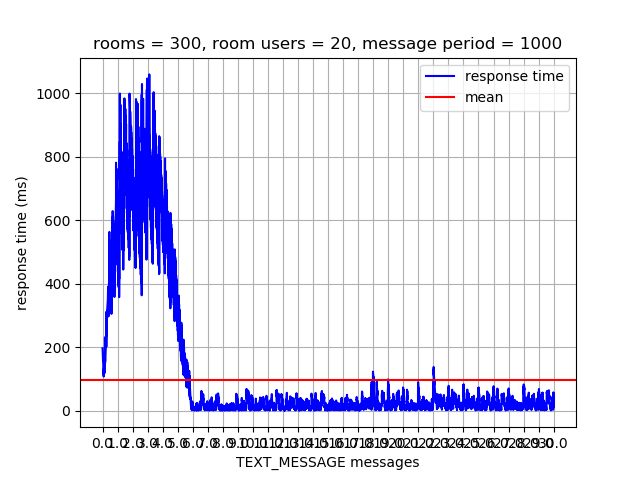
\includegraphics[scale=0.6,clip=true]{chat_r300_u20_m1000}
  \caption{Prueba de 300 rooms, 20 room users y 1000 msg period}
  \label{fig:chat_r300_u20_m100}
\end{figure}

Como podemos observar en la gráfica, al principio el tiempo de respuesta es mucho peor que el primer caso. El sistema tarda más tiempo en prepararse ya que son más usuarios enviando mensajes y conexiones WebSocket que mantener.

Algunos valores a destacar son:

\begin{itemize}
  \item \textbf{Media}: 97.3029789368 ms
  \item \textbf{Desviación típica}: 202.136129895 ms
  \item \textbf{Varianza}: 40859.015009 ms
  \item \textbf{Mensajes por segundo}: 373.925825854 msg/s
\end{itemize}

\subsection{Prueba de 400 salas, 20 usuarios por sala y 1 mensaje cada segundo}

En el último caso, a diferencia del anterior, se ha incrementado también el número de salas (400).

\begin{figure}[htp!]
  \centering
  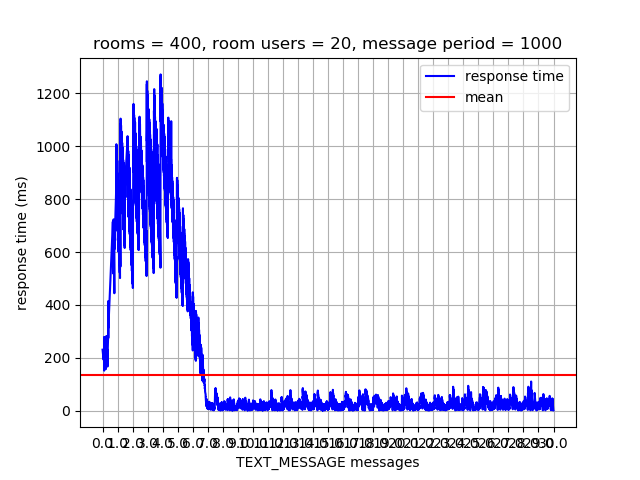
\includegraphics[scale=0.6,clip=true]{chat_r400_u20_m1000}
  \caption{Prueba de 400 rooms, 20 room users y 1000 msg period}
  \label{fig:chat_r400_u20_m1000}
\end{figure}

Como podemos observar en la gráfica, al principio el tiempo de respuesta es mucho peor que el segundo caso como era de esperar. Pero luego también consigue estabilizarse y dar buenos resultados.

Algunos valores a destacar son:

\begin{itemize}
  \item \textbf{Media}: 136.955281374 ms
  \item \textbf{Desviación típica}: 266.528534589 ms
  \item \textbf{Varianza}: 71037.4597502 ms
  \item \textbf{Mensajes por segundo}: 339.918519629 msg/s
\end{itemize}


%
% Conclusiones
%
\chapter{CONCLUSIONES\label{sec:conclusiones}}

TODO

\clearpage

\section{Conclusiones técnicas}

\subsection{Beneficios de las pruebas de software}

Las pruebas de software ahorran tiempo y dinero a una organización al reducir los costos de desarrollo y mantenimiento del software. Las pruebas de software crean garantías de estabilidad en el desarrollo de nuevas características.

El tiempo de desarrollo de las nuevas funciones se reduce especificando un conjunto de casos de prueba que la nueva característica debe cumplir para que se considere completa y entregable. Una vez que estos casos de prueba están en su lugar, los costos generales de mantenimiento se reducen.

Hay que tener bien claro los objetivos de las pruebas de software. Si bien es importante probar que los usuarios pueden usar la aplicación correctamente (iniciar sesión, guardar el estado de un objeto, etcétera), es igualmente importante probar que el sistema no se rompe cuando se envían datos incorrectos o se realizan acciones inesperadas.

\subsection{Beneficios de las pruebas de rendimiento}

Los problemas relacionados con el rendimiento en la producción afectan los ingresos que genera la aplicación y también es muy costoso de solucionar. Las pruebas de rendimiento no solo se realizan para medir en general el tiempo de respuesta de la aplicación, sino también para comprender el comportamiento del sistema con otras aplicaciones en el sistema.

Las pruebas de rendimiento, implementadas correctamente y realizadas a lo largo del ciclo de desarrollo, pueden reducir significativamente la cantidad de fallas experimentadas por una aplicación.

La pruebas de rendimiento han servido, entre otras cosas, para:

\begin{itemize}
  \item Demostrar que el sistema cumple con los criterios de rendimiento.
  \item Validar y verificar atributos de la calidad del sistema: escalabilidad, fiabilidad, uso de los recursos, etcétera.
  \item Medir qué partes del sistema o de carga de trabajo provocan que el conjunto rinda peor.
  \item Exponer memory leaks.
  \item Verificar que las políticas de recolección de basura (garbage collection) son adecuadas.
  \item Verificar que las agrupaciones de conexiones se están reciclando.
  \item Verificar que los manejadores de archivos se están reciclando.
\end{itemize}

\subsection{Beneficios de la arquitectura de las aplicaciones web}

El objetivo de separar las distintas funcionalidades en distintos servidores es aumentar la escalabilidad del sistema de cara a obtener un mayor rendimiento. Al separar las distintas funcionales en distintos servidores, cada uno de ellos se puede configurar de forma adecuada a los requisitos que presenta cada uno de ellos.

Por ejemplo, para el servidor web hace falta una máquina con una buena conexión a Internet, rápido pero sin grandes necesidades de almacenamiento. Sin embargo, para el servidor de bases de datos hace falta una máquina con mucha memoria y con un disco duro de alta capacidad de almacenamiento y rápido para mantener todos los datos.

Otra ventaja que se obtiene al separar las funcionalidades, es que al aislar la lógica de negocio y la lógica de datos en servidores separados que no están conectados directamente a Internet se aumenta el nivel de seguridad, ya que no es tan fácil acceder a ellos.

\subsection{Beneficios de las aplicaciones web en tiempo real}

Podemos afirmar que las aplicaciones web en tiempo real son necesarias. La razón principal no es la inmediatez en las interacciones, sino las mejoras en el rendimiento de la aplicación.

Los servidores web, aunque se encargan de gestionar los mensajes de los clientes, se ahorran los DDoS involuntarios por demasiados clientes conectándose a la vez. El tráfico de red disminuye, algo bastante conveniente con las actuales tarifas para móviles, y las aplicaciones sólo consumen CPU cuando es realmente necesario, y no cada periodo de tiempo de forma fija.

Es cierto que el tiempo real es en parte la excusa perfecta para ver hasta dónde puede llegar la tecnología, pero eso no quita que no nos pueda resultar útil. Podemos encontrar muchos ejemplos de aplicaciones que hacen uso de tiempo real y que son bastante útiles.

\subsection{Beneficios de los WebSockets}

Resulta que hay un gran abismo entre implementar el protocolo WebSocket en una aplicación web, y llevar esa implementación a producción. Algunas de las librerías populares podrían matar tu servidor inmediatamente si la cantidad de conexiones aumenta, en otros casos empiezas a notar pérdida de memoria por cada conexión WebSocket que no fue propiamente desconectada.

Los problemas que pueden producirse en producción usando WebSockets debería medirse a través de las pruebas de rendimiento.

Si bien, la implementación en producción de los WebSockets trae consigo enormes problemas, también presenta los mejores beneficios:

\begin{itemize}
  \item Tiempo de respuesta más rápido que otros mecanismos, ideal para chats.
  \item Aplicaciones más rápidas, ya que la comunicación queda permanentemente abierta.
  \item Y modernas, con excelentes herramientas para backend y frontend.
\end{itemize}

\subsection{Beneficios de las aplicaciones web en Node.js}

Cuando Node.js se introdujo en la comunidad tecnológica en 2009 como una herramienta para crear aplicaciones web escalables en el lado del servidor, se presentaron muchos beneficios que incluyen, entre otros, el uso del modelo de entrada/salida no bloqueante dirigido por eventos y la programación asíncrona de un solo hilo.

Node.js te permite escribir el mismo idioma tanto para tu frontend como para tu backend, ahorrandote el estrés de aprender un nuevo idioma para alguna implementación simple y también te ayuda a mantener el mismo patrón de diseño en todo momento.

En este proyecto hemos optado por crear el backend con Node.js, ya que este ofrece más posibilidades y es de más bajo nivel que otros lenguajes. Además, ofrece un rendimiento impecable y como decíamos antes, el proceso de desarrollo es ágil debido a la facilidad de inclusión de paquetes para crear funcionalidad específica mediante npm. Si queremos crear un servicio RESTful con capacidades en tiempo real, la combinación de Express.js con WebSockets nos permite hacerlo de manera fácil y rápida.

\subsection{Memory leaks en Node.js}

La pérdida de memoria es muy común en las aplicaciones de Node.js, especialmente en las de gran escala con tráfico razonable, y muchas empresas grandes la han sufrido.

Una aplicación de Node.js se inicia sólo una vez, no para cada solicitud entrante. Esto hace que el manejo peticiones sea más rápido, ya que solo hace la lógica para cada petición. sin necesidad de trabajo repetitivo, también ahorra los recursos necesarios para este proceso de iniciación.

Pero esto conlleva un precio, que tienes que ocuparse del uso de la memoria de la aplicación, ya que consumirá la memoria continuamente durante su tiempo de ejecución y, si no se maneja el uso de la memoria de manera eficiente, puede agotarse la memoria.

\subsubsection{Causas comunes de memory leak}

Teniendo en cuenta la gestión de memoria en Node.js, podemos definir tres de las causas más comunes de pérdida de memoria que deberíamos tener cuidado al usarlas en un código:

\begin{itemize}
  \item Variables globales. Dado que tienen una ruta directa al nodo raíz, permanecerán en la memoria mientras la aplicación se esté ejecutando, por lo que se debe tener cuidado al configurar las variables globales y la cantidad de datos que se establecerá en ellas.
  \item Referencias múltiples. La configuración de varias referencias al mismo objeto también puede causar problemas, ya que puede eliminar una referencia y olvidar la otra, lo que mantendrá el objeto en cuestión ocupando espacio.
  \item Closures. En los closures, simplemente mantiene las referencias a los objetos que se utilizarán más adelante. esta característica tiene muchas ventajas, pero si se usa sin precaución, puede causar grandes problemas, ya que estas referencias mantendrán a los objetos en la pila y estos pueden ser grandes.
\end{itemize}

\subsubsection{V8 Inspector y Chrome DevTools}

Existen muchas herramientas y bibliotecas que se utilizan para detectar memory leaks en Node.js, todas siguen el mismo concepto para detectar memory leaks de comparar diferentes volcados de pila (heap dump) y verificar los resultados, e intentan forzar la ejecución del garbage collector antes de tomar cualquier head dump para hacer asegurarse de que la pérdida es real.

Una herramienta muy importante, desde mi punto de vista, es el V8 Inspector. Muy útil, especialmente cuando se usa con Chrome DevTools en la fase de desarrollo, ya que te permite monitorear el rendimiento de uso de la memoria para verificar si hay alguna pérdida potencial en el código y encontrar dónde podría ocurrir exactamente esa pérdida.

La diferencia entre dos volcados de pila es un indicador de la cantidad de pérdida de memoria en una aplicación.

\subsection{Beneficios de los contenedores de Docker}

A efectos técnicos, Docker es una tecnología de virtualización “ligera” en el sentido de que, en lugar de replicar una máquina virtual completa, únicamente se virtualiza los servicios del contenedor \cite{docker3}.

Docker es una herramienta diseñada para beneficiar tanto a desarrolladores como a testers.

En el caso de los desarrolladores, el uso de Docker hace que puedan centrarse en desarrollar su código sin preocuparse de si dicho código funcionará en la máquina en la que se ejecutará.

Por eso Docker también es muy bueno para el testing, para tener entornos de pruebas. Por un lado, es muy sencillo crear y borrar un contenedor, además de que son muy ligeros, por lo que podemos ejecutar varios contenedores en una misma máquina.

\section{Implantación real del prototipo}

TODO

\subsection{Virtualización}

Dependiendo del escenario, una u otra opción de virtualización puede ser la más apropiada.

La tecnología de contenedores ayuda a obtener mayor flexibilidad y portabilidad pues las aplicaciones se pueden ejecutar, ya sea en las instalaciones físicas o en la nube.

El nivel de paquetización consigue que una aplicación pueda ser trasladada de un ambiente a otro con mínimo o nulo impacto, permitiendo que en escenarios de alta carga el sistema pueda escalar clonando nuevas instancias de la aplicación muy rápido.

Esto además beneficia a la parte de sistemas, ya que los contenedores son más ligeros que las máquinas virtuales, se reduce el número de máquinas necesarias para tener un entorno.

\subsection{Instalación on-premise}

El término on-premise se refiere al tipo de instalación de una solución de software. Esta instalación se lleva a cabo dentro de la infraestructura de la empresa, asumiendo la responsabilidad de la seguridad, la disponibilidad y la gestión del software. Por lo que debe tener un departamento que dedique parte de sus recursos a la gestión de la infraestructura in situ. El proveedor de la solución software también puede proporcionar servicios de integración y soporte post-venta.

La instalación on-premise suele estar más asociada a empresas que buscan resultados profesionales, evitando tomar riesgos con servidores sobrecargados o revelación de datos internos.

\subsubsection{Ventajas de la instalación on-premise}

Aunque la inversión inicial sea más arriesgada, ofrece ventajas como una mayor control del software. Por ello, hay que tener en cuenta algunos aspectos a la hora de decidir una instalación on-premise:

\begin{itemize}
  \item Coste. Reduce el precio de una solución a largo plazo, aunque la inversión inicial puede ser más arriesgada.
  \item Seguridad. La seguridad de los datos está en las manos de la empresa.
  \item Personalización. Facilidad de personalización.
  \item Implementación. La empresa tiene más control sobre el proceso de implementación, pero este proceso puede tomar más tiempo.
\end{itemize}


%
% Conclusiones
%
\chapter{LÍNEAS FUTURAS\label{sec:lineasfuturas}}

TODO

\clearpage

\section{Servicios avanzados de PEMEA}

Los primeros resultados del proyecto, junto con las pruebas realizadas, confirman el poder de PEMEA para proporcionar:

\begin{itemize}
  \item Ciudadanos con acceso a servicios de emergencia en cualquier lugar de Europa utilizando sus apps locales en roaming.
  \item Los PSAPs con la información correcta (ubicación precisa, idioma de la persona que llama, contactos de ICE, etcétera), independientemente de la app que la persona esté utilizando.
\end{itemize}

En una segunda etapa, los servicios de emergencia se beneficiarán de los servicios avanzados de PEMEA, como geolocalización, compartición de imágenes y vídeos, o comunicación en tiempo real, para mejorar el acceso a los ciudadanos que presentan algún tipo de discapacidad y personas dependientes.

Deveryware ya ha invertido en este campo 3 años de investigación y experimentación.

\section{Chatbots}

Hoy en día las apps de mensajería están convirtiéndose en uno de los servicios más utilizados por los usuarios de dispositivos móviles. Por esta razón, varios sectores están incorporando estos canales a sus modelos de negocio, un servicio que no estará controlado por personas, sino por robots.

En este sentido, tanto editores como apps de mensajería están centrando todos sus esfuerzos en el desarrollo de softwares de inteligencia artificial para crear chatbots, es decir, bots capaces de entablar conversaciones con los usuarios.

Un bot es un software de inteligencia artificial diseñado para realizar una serie de tareas por su cuenta y sin la ayuda del ser humano.

Los chatbots son un tema candente en estos días. Los conjuntos de herramientas disponibles han permitido a muchas empresas integrar con éxito la tecnología de chatbot en sus sistemas empresariales, ahorrando tiempo y dinero.

Una de las grandes ventajas de los chatbots es que, a diferencia de las aplicaciones, no se descargan, no es necesario actualizarlos y no ocupan espacio en la memoria del teléfono.

Otros lugares en los que han estado en funcionamiento en los últimos años ha sido en chats como Facebook Messenger o en aplicaciones de mensajería instantánea como Telegram o Slack. En estas últimas los chatbots estaban incorporados como si fueran un contacto más.

Los chatbots de inteligencia artificial, el futuro de las apps de mensajería.

\subsection{Azure V3 Translator Text}

Uno de los desafíos que enfrentan los equipos de desarrollo al crear un nuevo chatbot es cómo manejar la traducción de idiomas para un chatbot implementado globalmente. Debido a los aspectos dinámicos de una conversación de chat, la localización de aplicaciones es difícil, en el mejor de los casos.

Lo que necesita un chatbot global es una forma de detectar el idioma entrante del usuario, traducirlo al idioma que su bot entiende y luego traducir la respuesta del bot al idioma de entrada original del usuario. Todo esto debe suceder dinámicamente y sobre la marcha.

La API del Translator Text de los Servicios Cognitivos de Microsoft proporciona las herramientas para lograr esto.

Para realizar la detección y traducción de idiomas, necesitamos utilizar la API del Translator Text. La API del Translator Text puede realizar la detección automática de idiomas, la traducción, la transliteración y las búsquedas de diccionarios bilingües. Admite más de 60 idiomas y Microsoft continúa agregando más.

Al escribir un chatbot que podría usarse en cualquier parte del mundo, las funciones le brindarán a su aplicación el soporte que necesita para comunicarse con cualquier usuario en su idioma nativo.


%
% Página en blanco
%
\cleardoublepage

%
% Bibliografía
%
\printbibliography[heading=bibintoc]

% No expandir elementos para llenar toda la página
\raggedbottom

%
% Apéndices
%
\appendix
\cleardoublepage
\addappheadtotoc
\appendixpage

%
% TODO: Apéndices del TFG
%
\chapter{Ejemplos de bloques y comandos útiles en LaTeX\label{sec:ejemplos}}
\section{Ejemplo de sección}

%
% Breve guía de comandos útiles para la memoria
%

% Citar una referencia
La DARPA creó el protocolo de Internet \cite{ipv4sta}.

% Citar una referencia
La DARPA creó el protocolo de YEAH Internet \cite{ipv2sta}.

% Citar un elemento del glosario
Citamos el acrónimo \gls{FPGA}.

% Citar un elemento del glosario (primera letra en may´usculas)
\Gls{bitstream} es una secuencia de bits.

% Insertar una imagen con pie de página
\begin{figure}[htp!]
  \centering
  \includegraphics[width=0.75\textwidth,clip=true]{logo_politecnica}
  \caption{Logo de la Universidad Politécnica de madrid.}
  \label{fig:logo_uam}
\end{figure}

% Referenciar una etiqueta (label)
La figura~\ref{fig:logo_uam} se utiliza en la portada.

% Nueva página
\clearpage

% Añadir código fuente sin líneas
\begin{lstlisting}[label=algoritmo:quicksort,language=C,frame=single,caption=Algoritmo de ordenación Quicksort]
#include <stdio.h>

void quick_sort (int *a, int n) {
    int i, j, p, t;
    if (n < 2)
        return;
    p = a[n / 2];
    for (i = 0, j = n - 1;; i++, j--) {
        while (a[i] < p)
            i++;
        while (p < a[j])
            j--;
        if (i >= j)
            break;
        t = a[i];
        a[i] = a[j];
        a[j] = t;
    }
    quick_sort(a, i);
    quick_sort(a + i, n - i);
}
\end{lstlisting}

% Bloque de código inseparable
\begin{code}
#include <stdio.h>

void quick_sort (int *a, int n) {
    int i, j, p, t;
    if (n < 2)
        return;
    p = a[n / 2];
    for (i = 0, j = n - 1;; i++, j--) {
        while (a[i] < p)
            i++;
        while (p < a[j])
            j--;
        if (i >= j)
            break;
        t = a[i];
        a[i] = a[j];
        a[j] = t;
    }
    quick_sort(a, i);
    quick_sort(a + i, n - i);
}
\end{code}

% Fórmula dentro de una línea de texto
La ecuación de Euler ($e^{ \pm i\theta } = \cos \theta \pm i\sin \theta$) es citada frecuentemente como un ejemplo de belleza matemática.

% Fórmula independiente
\begin{equation}\label{eq:pythagoras}
a^2 + b^2 = c^2
\end{equation}


% Fin del documento
\end{document}
